\chapter{Inclusive Jet \Xs{s}}
\label{chap:forward-inclusive}

\chapterquote{It's not exclusive, but inclusive, which is the whole spirit of
jazz.}{Herbie Hancock}

\section{Introduction}
As discussed in \SectionRef{sec:bg-theory:jets_in_hadron_colliders}, jet production
is the dominant high \pT process at the \LHC. Jet \xs{s} are important
observables in high-energy particle physics and are one of the first measurements
that can be performed in a hadron collider experiment. These \xs{s} are
an important tool for understanding the strong interaction, in particular through
providing precise measurements of \alphaS. In addition to testing \QCD in a
new kinematic regime, the data also provide sensitivity to different parton distribution
functions (PDFs) in a region where they are currently poorly constrained.

This analysis presents inclusive double-differential jet \xs{s}; studied
as a function of jet \pT and \rap. The measurement covers $\unit{20}{\GeV} \leq \pT < \unit{1.5}{\TeV}$
in the rapidity range $\absRap < 4.4$. The results are compared to theoretical predictions
from next-to-leading order \QCD corrected for non-perturbative effects, as well as
to next-to-leading order \MC simulations. The rapidity slices used in the measurement
have boundaries which follow the calorimeter geometry.

\section{\Xs Definition}
\label{sec:forward-inclusive:cross_section_definition}
Clearly, jet \xs{s} can only be defined for a specific jet algorithm;
here \xs{s} have been calculated for the \ATLAS standard: \akt jets with
$R=0.4$ and $R =0.6$ (see \SectionRef{bg-theory:recombination_algorithms} and
\SectionRef{sec:analysis-tools:jet_reconstruction}). The jet \xs measurements
are corrected for all experimental effects (see \SectionRef{sec:analysis-tools:unfolding}),
and so refer to the ideal particle level final state of a proton-proton
collision~\cite{Buttar:2008:toolsandjets}. In the \MC, particle level jets are
identified using the same jet algorithms applied to data, using stable particles,
all those with a proper lifetime longer than \unit{10}{\pico\second}, as their
input. This definition includes muons and neutrinos from decaying hadrons which
cannot be included in calorimeter jets reconstructed in data.

\section{Event Selection}
Following the outline in \SectionRef{sec:analysis-tools:data_selection}, events
are required to belong to a good run and to have at least one good primary
vertex. All jets in the event which satisfy $\pT \geq \unit{20}{\GeV}$ and
$\absRap < 4.4$ are retained unless they are flagged as ``bad'' or ``ugly'' by
the standard medium jet cleaning cuts (see \SectionRef{sec:analysis-tools:jet_cleaning}).
Each jet is then assigned a specific, fully-efficient trigger which depends on
its transverse momentum and rapidity, as well as the run period that the event
belongs to. For the jet to contribute towards the inclusive \xs, this trigger must be passed. All jets which pass their trigger are retained,
with a weight reflecting the amount of luminosity seen by the trigger, which, due
to prescaling, is usually less than then the total luminosity recorded by \ATLAS.

\section{Trigger Strategy}
\label{sec:forward-inclusive:trigger}
This measurement uses three different trigger systems (see \SectionRef{sec:detector:trigger}):
the Minimum Bias Trigger Scintillators (MBTS) are used to select events
containing jets with $20 \leq \pT < \unit{60}{\GeV}$, the central jet triggers are
used for the remainder of the phase space region $\absRap<3.6$ while the forward
jet triggers are used for jets with $3.2 \leq \absRap < 4.9$. In the region $3.2 \leq \absRap < 3.6$
a combination of central and forward jet triggers is used. The L1\_MBTS\_1
trigger has been demonstrated to have a negligible inefficiency in selecting
the low \pT events for which it is used here.

For this measurement, the rapidity interval $\absRap < 4.4$ was divided into seven
bins: the central bins with $\absRap < 2.8$, the HEC-FCAL transition bin with $2.8 \leq \absRap < 3.6$
and the forward bin with $\absRap \geq 3.6$. As discussed in \SectionRef{sec:analysis-tools:jet_selection_evolution},
increasing instantaneous luminosity throughout 2010 means that the lowest prescaled
fully efficient trigger in each \pT bin changes over time.

\TableRangeRef{tab:forward-inclusive:TriggersCentral}{tab:forward-inclusive:TriggersForward}
summarise the triggers that are used in each \pT bin of the \xs measurement
as a function of the data taking period. For the central bins, these are central jet
triggers and for the forward bin, forward jet triggers. In both cases, certain
bins are augmented by data taken using the L1\_MBTS\_1 trigger. It is confirmed
that all of these triggers are over 99\% efficient in these regions.

\begin{table}
\begin{center}
  \begin{tabular}{ l l l l l }
             & \multicolumn{2}{c}{Period A*--F}         & \multicolumn{2}{c}{Period G--I}               \\
                    \cmidrule(lr){2-3}                         \cmidrule(lr){4-5}
  \pT range  & Central       & Central crack            & Central           & Central crack             \\
  {[}\GeV{]} & $\absRap<2.8$ & $1.2 \leq \absRap < 2.1$ & $\absRap<2.8$     &  $1.2 \leq \absRap < 2.1$ \\
             & except crack  &                          & except crack      &                           \\
  \midrule
  60--80     & L1\_J5        &  L1\_J5                  & EF\_j20\_jetNoEF  & EF\_j20\_jetNoEF          \\
  80--110    & L1\_J15       &  L1\_J5                  & EF\_j35\_jetNoEF  & EF\_j20\_jetNoEF          \\
  110--160   & L1\_J30       &  L1\_J15                 & EF\_j50\_jetNoEF  & EF\_j35\_jetNoEF          \\
  160--210   & L1\_J55       &  L1\_J30                 & EF\_j75\_jetNoEF  & EF\_j50\_jetNoEF          \\
  210--260   & L1\_J75       &  L1\_J55                 & EF\_j95\_jetNoEF  & EF\_j75\_jetNoEF          \\
  260--310   & L1\_J95       &  L1\_J75                 & EF\_L1J95\_NoAlg  & EF\_j95\_jetNoEF          \\
  310--400   & L1\_J95       &  L1\_J95                 & EF\_L1J115\_NoAlg & EF\_L1J95\_NoAlg          \\
  400+       & L1\_J95       &  L1\_J95                 & EF\_L1J115\_NoAlg & EF\_L1J115\_NoAlg         \\
  \end{tabular}
  \caption{The trigger chains used for the inclusive jet analysis in the region
           $\absRap<2.8$. The L1\_MBTS\_1 trigger is used for the $20 \leq \pT < \unit{60}{\GeV}$
           over the range $\absRap<2.8$. Due to mistimings in the Level-1 central
           jet trigger hardware, L1\_MBTS\_1 was also used to trigger all jets before
           run 152777. The period after this timing change is here denoted as ``A*''.}
  \label{tab:forward-inclusive:TriggersCentral}
\end{center}
\end{table}

\begin{table}
\begin{center}
  \begin{tabular}{ l l l l }
  \pT range $[\GeV]$ & Period A--C & Period E5--F & Period G--I       \\
  \midrule
  20--30             & L1\_MBTS\_1 & n/a          & n/a               \\
  30--45             & n/a         & L1\_FJ10     & n/a               \\
  45--60             & n/a         & L1\_FJ10     & n/a               \\
  60--80             & n/a         & L1\_FJ10     & EF\_fj30\_jetNoEF \\
  80--110            & n/a         & L1\_FJ30     & EF\_fj30\_jetNoEF \\
  110--160           & n/a         & L1\_FJ55     & EF\_fj50\_jetNoEF \\
  160--210           & n/a         & L1\_FJ55     & EF\_fj75\_jetNoEF \\
  210--260           & n/a         & L1\_FJ55     & EF\_fj75\_jetNoEF \\
  260+               & n/a         & L1\_FJ55     & EF\_fj75\_jetNoEF \\
  \end{tabular}
  \caption{The trigger chains used for the inclusive jet analysis in the forward
           region, $3.6 \leq \absRap < 4.4$. The first four periods (A--D) could not
           be used, as the forward jet trigger had not yet been commissioned, while
           additional problems made it unreliable for subperiods E1--4. L1\_MBTS\_1
           was found to be fully efficient for forward jets and hence was used in
           early periods to trigger low \pT forward jets.}
  \label{tab:forward-inclusive:TriggersForward}
\end{center}
\end{table}

\subsection{Trigger Strategy in the Transition Region}
\label{sec:forward-inclusive:transition_triggers}
A jet is accepted as having passed its particular inclusive trigger requirement if
at least one jet in the event has passed that trigger. Due to the reduced
\pseudorap-granularity available in the trigger system, it is therefore possible
for jets in the forward region to belong to an event in which only central trigger
chains have fired, or \emph{vice versa}. Events of this type will predominantly fall into
the HEC-FCAL transition region, $2.8 \leq \absRap < 3.6$. Additionally, it is possible
that jets in this region might trigger both the central and forward trigger systems.
It can be seen in \FigureRef{fig:forward-inclusive:eta_efficiency_akt} that, when taking
central and forward triggers with the same \ETEM threshold, the logical OR of the
two triggers is fully efficient across this transition region although neither trigger
is on its own.

\begin{figure}[htpb]
  \subfloat[\Akt $R=0.4$ jets, 2010 data]{
    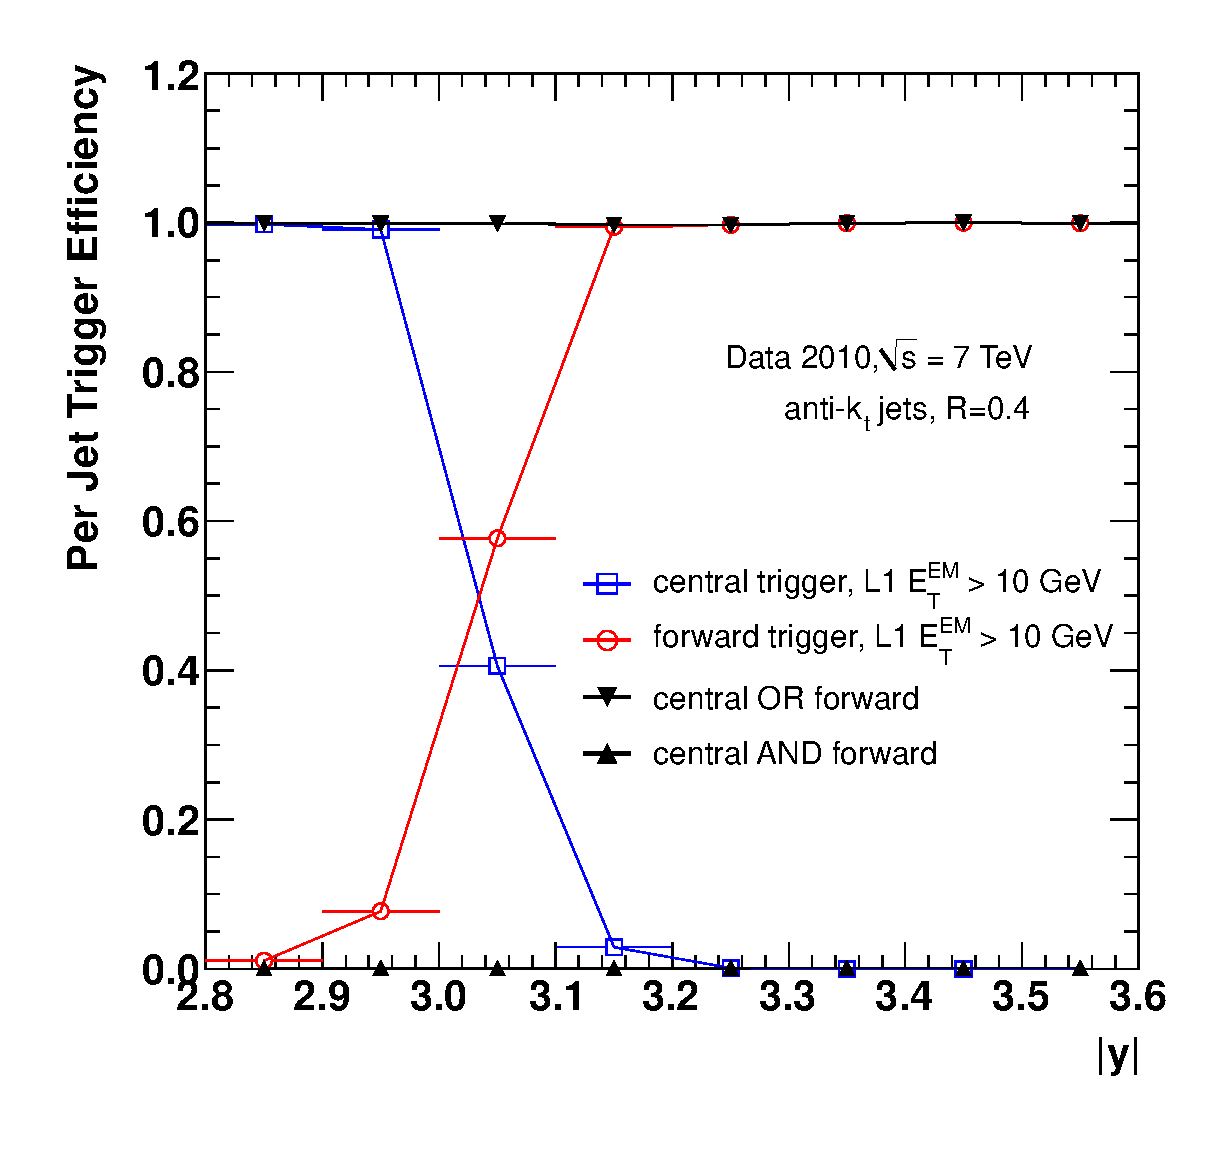
\includegraphics[width=\smallfigwidth]{chapters/forward-inclusive/TriggerEfficiency.akt4.data.eps} %eta_efficiency_akt4.eps}
    \label{fig:forward-inclusive:eta_efficiency_data_akt4}}
  \quad
  \subfloat[\Akt $R=0.6$ jets, 2010 data]{
    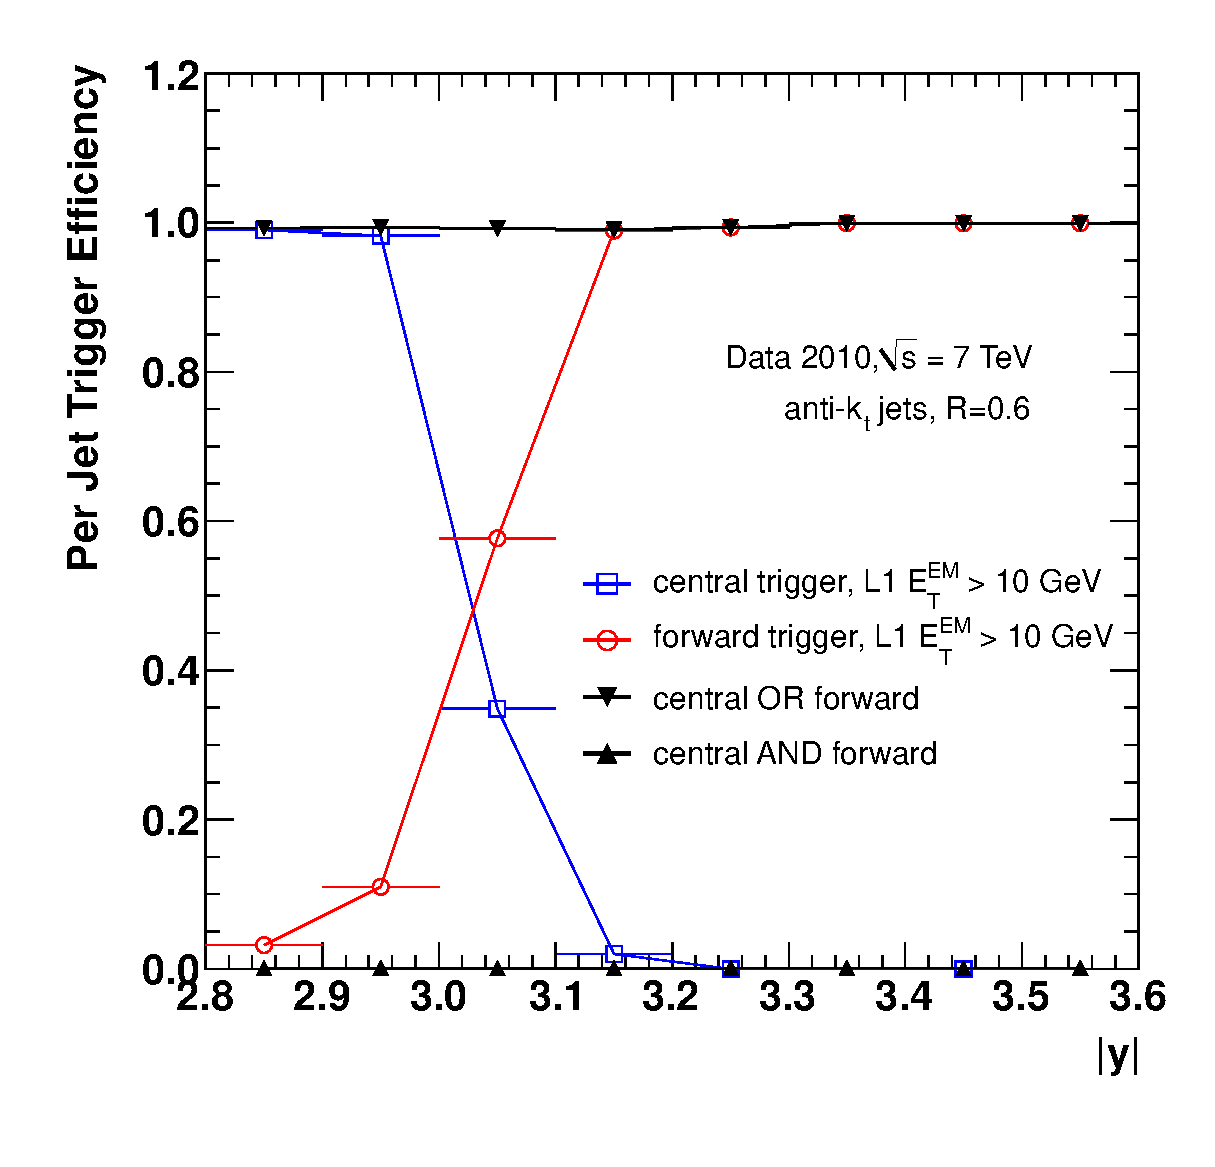
\includegraphics[width=\smallfigwidth]{chapters/forward-inclusive/TriggerEfficiency.akt6.data.eps} %eta_efficiency_akt6.eps}
    \label{fig:forward-inclusive:eta_efficiency_data_akt6}}
  \\
  \subfloat[\Akt $R=0.4$ jets, \Pythia]{
    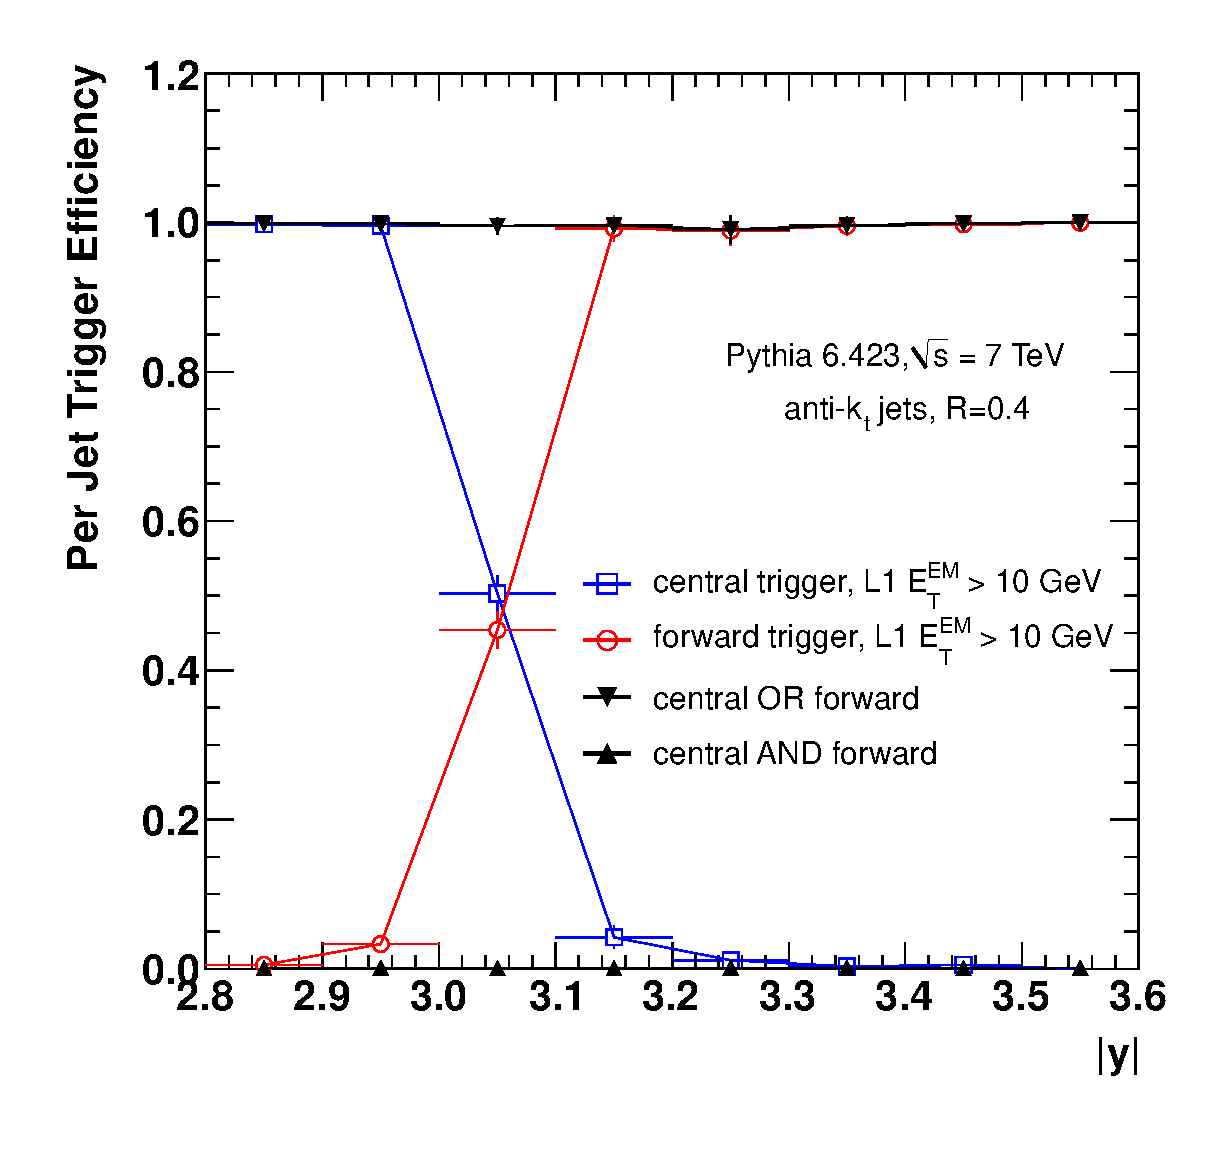
\includegraphics[width=\smallfigwidth]{chapters/forward-inclusive/TriggerEfficiency.akt4.pythia.eps} %eta_efficiency_akt4.eps}
    \label{fig:forward-inclusive:eta_efficiency_pythia_akt4}}
  \quad
  \subfloat[\Akt $R=0.6$ jets, \Pythia]{
    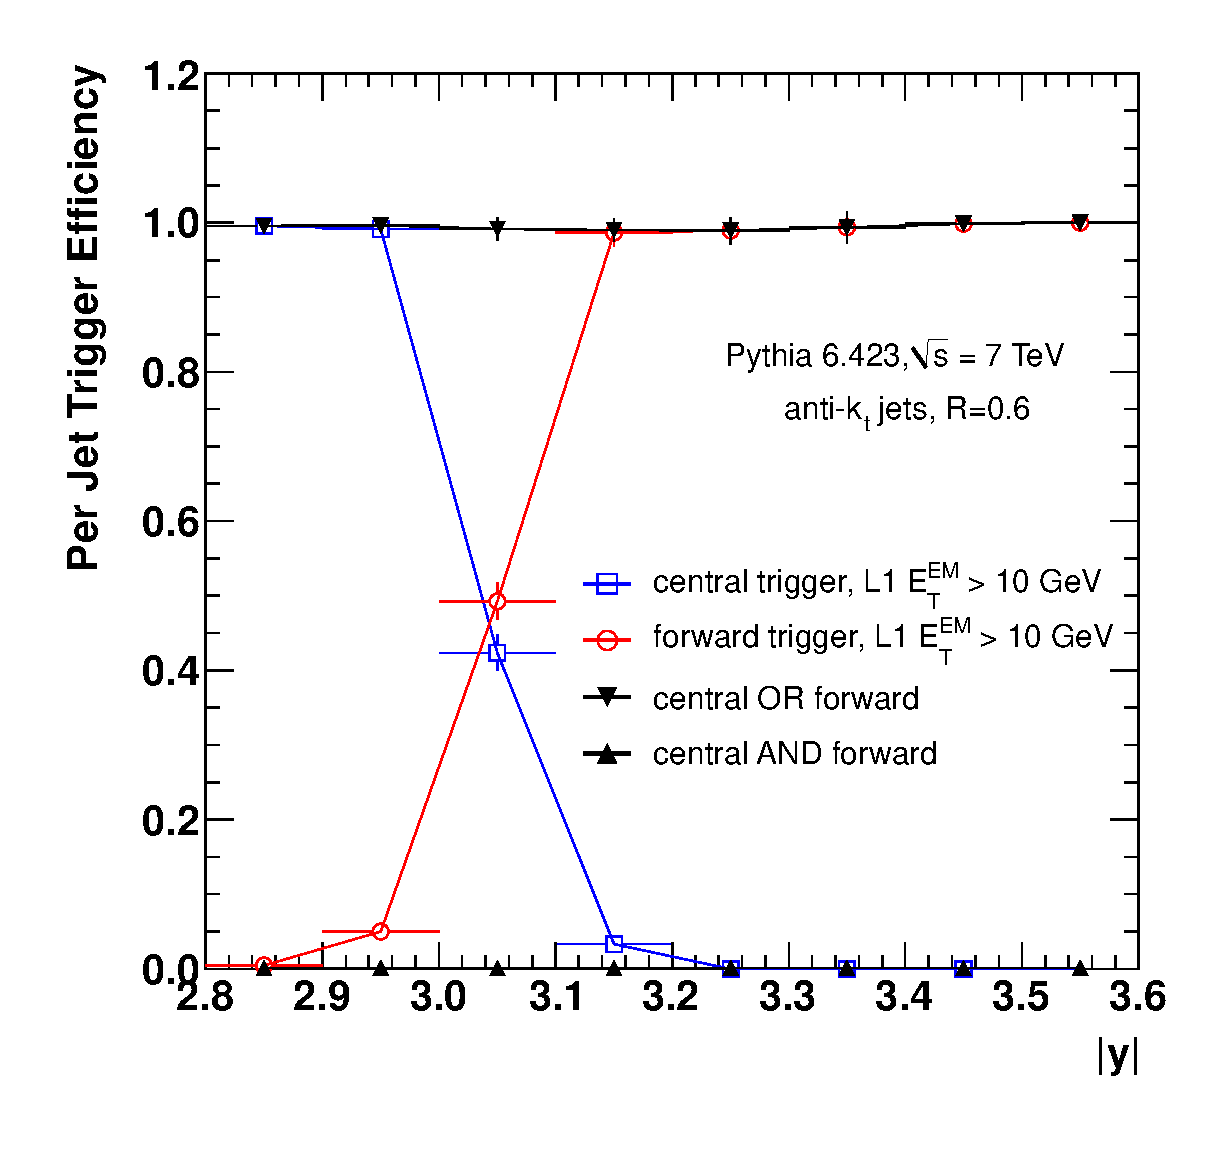
\includegraphics[width=\smallfigwidth]{chapters/forward-inclusive/TriggerEfficiency.akt6.pythia.eps} %eta_efficiency_akt6.eps}
    \label{fig:forward-inclusive:eta_efficiency_pythia_akt6}}
  \caption{Efficiency of the central and forward trigger signatures J10 and FJ10,
           their AND and their OR, as a function of rapidity, \rap, of the offline jet.
           Trigger efficiency is shown in data (top) and in \MC (bottom) while
           \akt $R=0.4$ jets (left) and \akt $R=0.6$ jets (right) are also considered
           separately.}
  \label{fig:forward-inclusive:eta_efficiency_akt}
\end{figure}

Sample turn-on curves for the central OR forward combination can be
seen in \FigureRef{fig:forward-inclusive:transition_bin_trigger_efficiencies}, demonstrating
that this combination is fully efficient at sufficiently high jet \pT. \TableRef{tab:forward-inclusive:TriggersTransition}
summarises the triggers that are used in each \pT bin of the \xs measurement
as a function of the data taking period.

\begin{figure}[htpb]
  \subfloat[L1 efficiency, \akt $R=0.4$ jets]{
    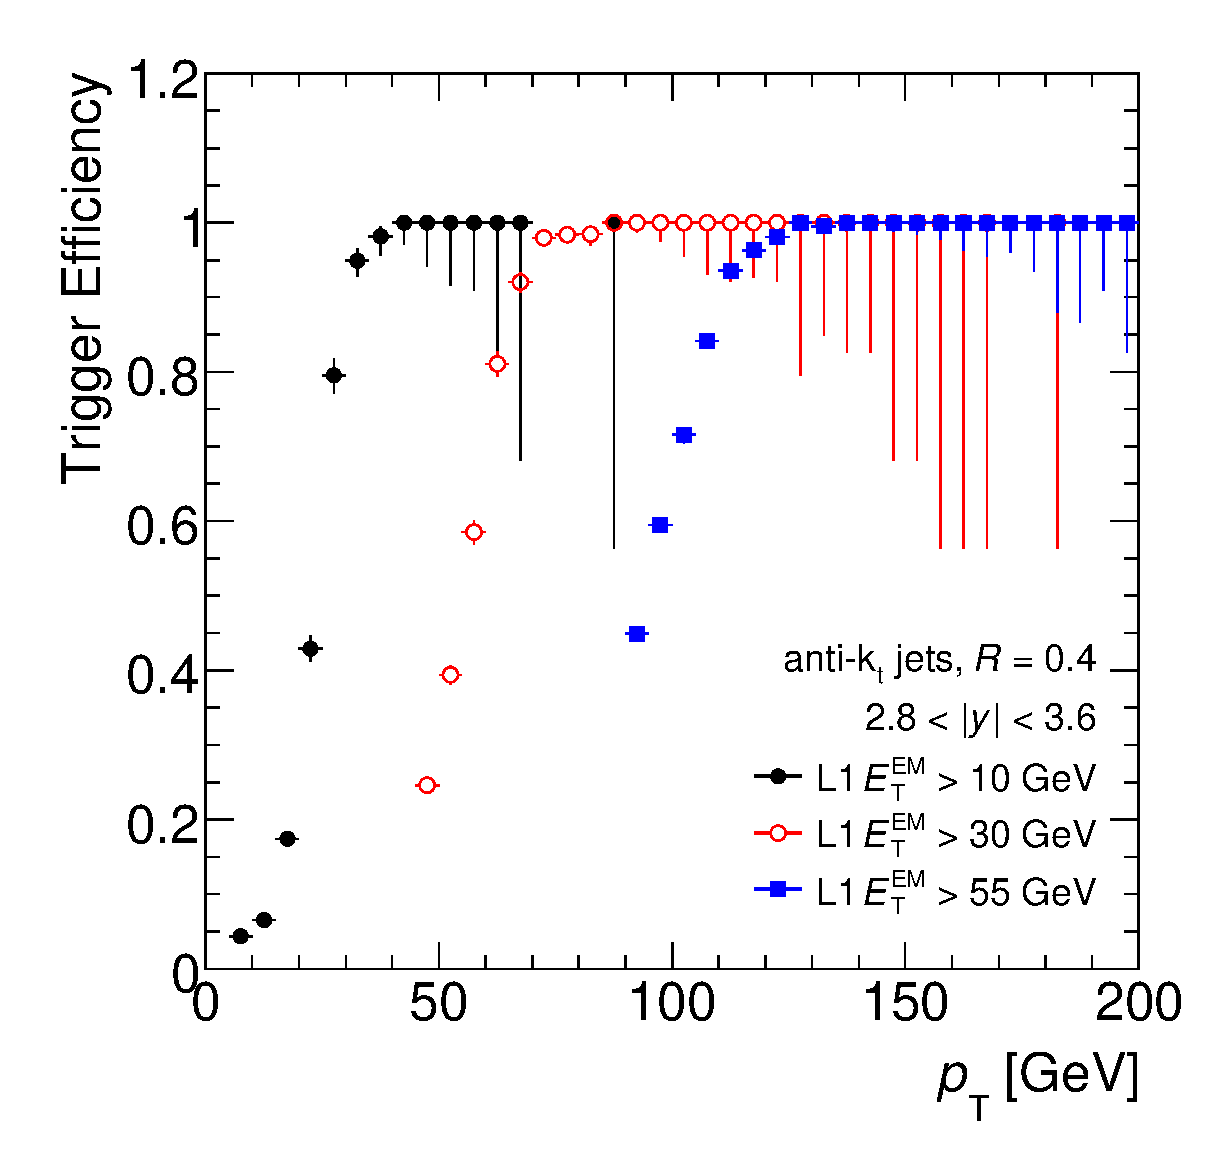
\includegraphics[width=\smallfigwidth]{chapters/forward-inclusive/transition_bin_triggers_L1_akt4.eps}
    \label{fig:forward-inclusive:transition_bin_triggers_L1_akt4}}
  \quad
  \subfloat[L1 efficiency, \akt $R=0.6$ jets]{
    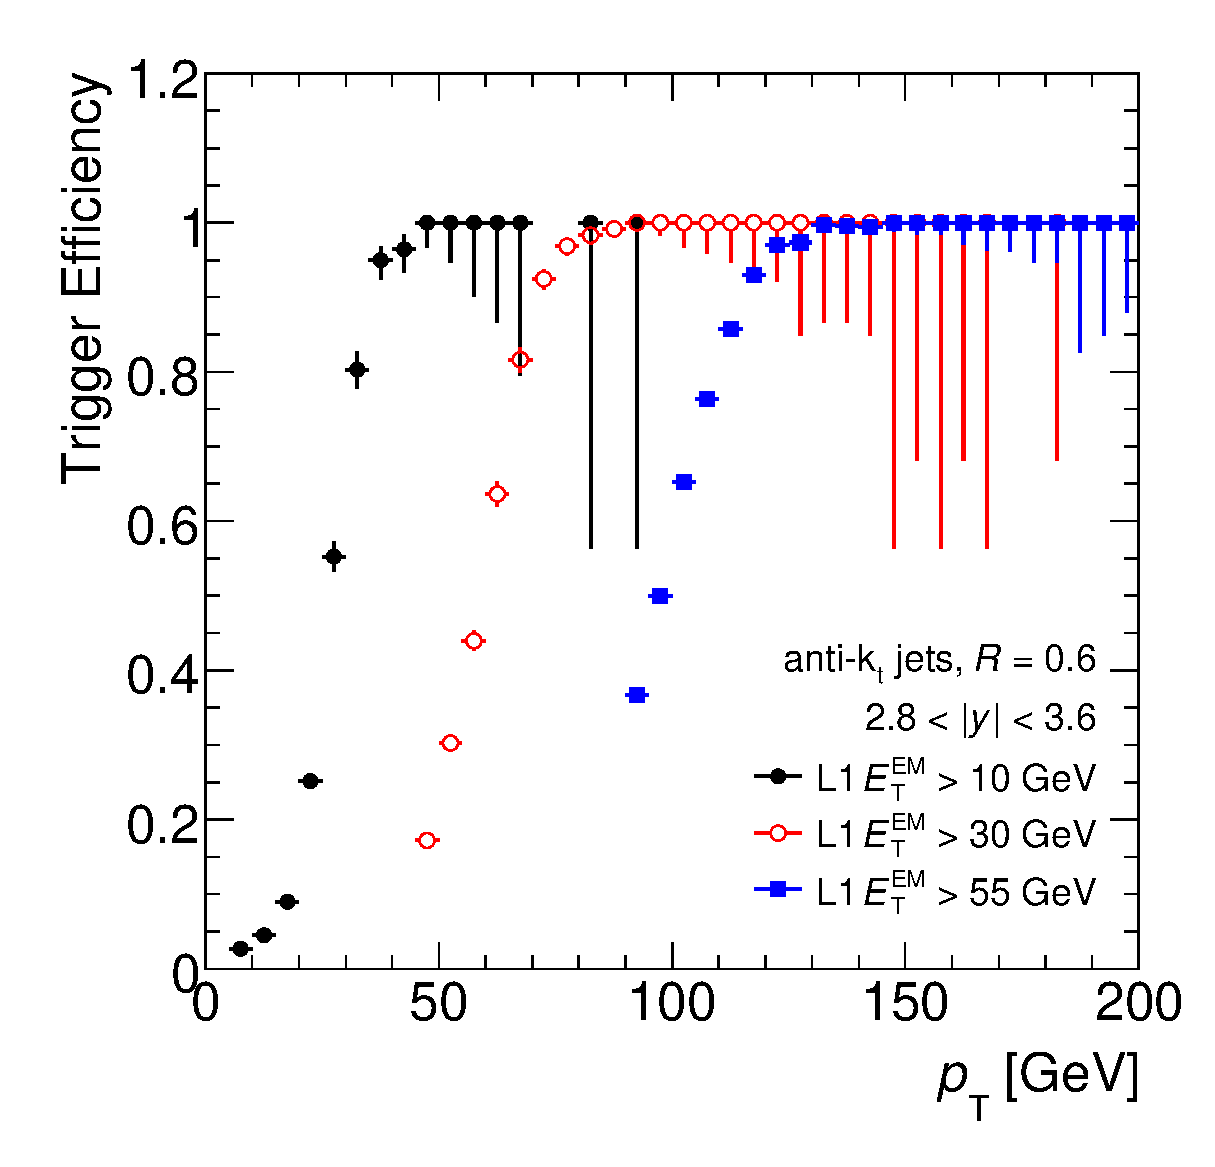
\includegraphics[width=\smallfigwidth]{chapters/forward-inclusive/transition_bin_triggers_L1_akt6.eps}
    \label{fig:forward-inclusive:transition_bin_triggers_L1_akt6}}
  \\
  \subfloat[L1+L2 efficiency, \akt $R=0.4$ jets]{
    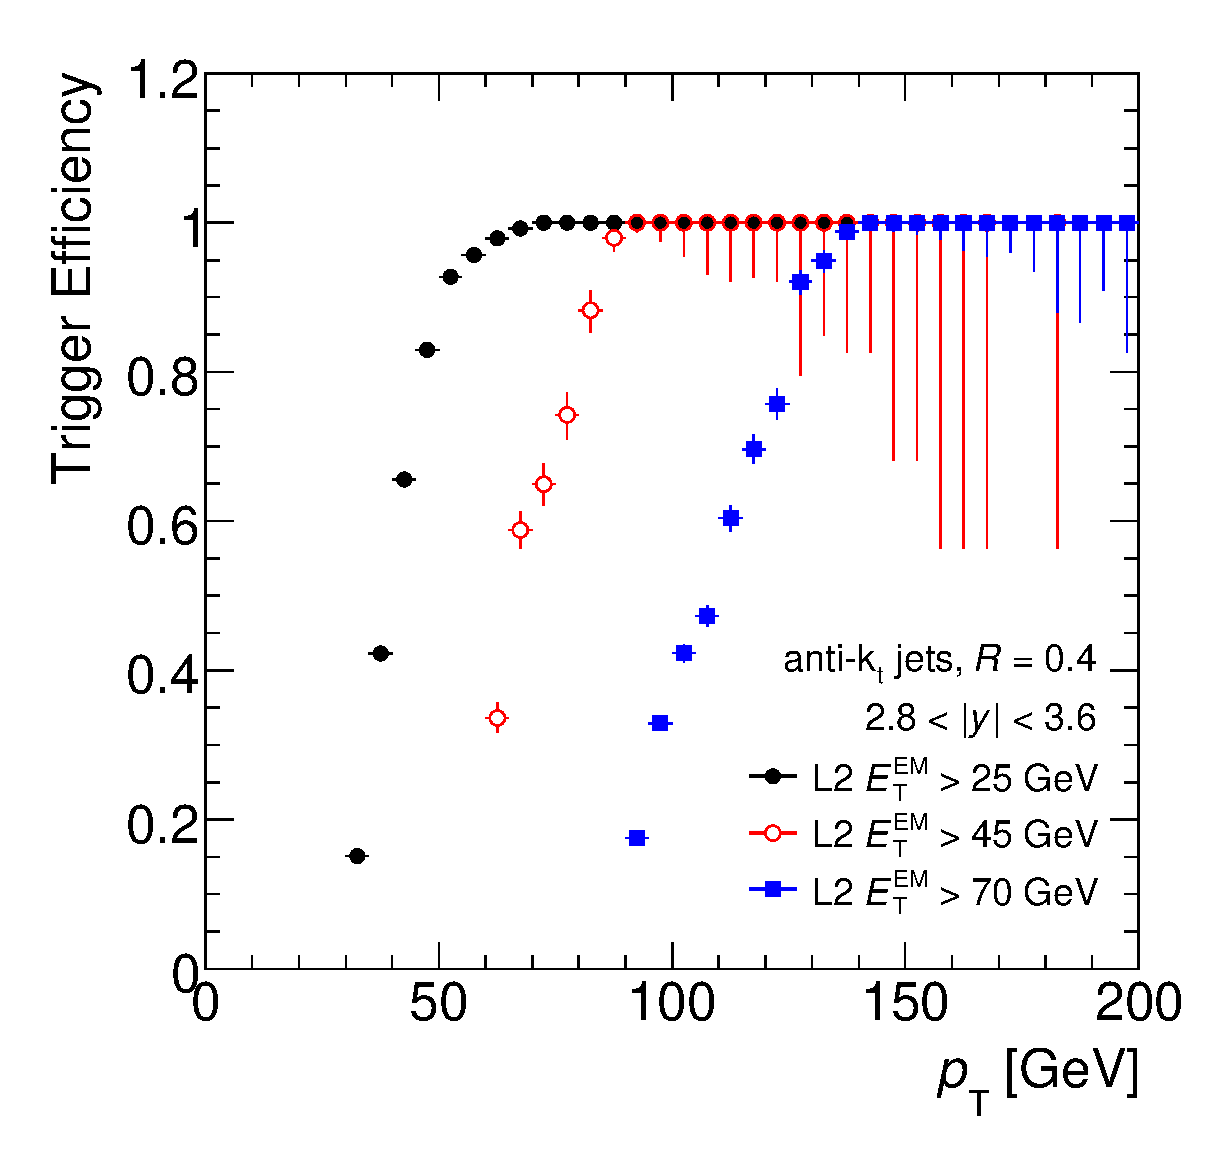
\includegraphics[width=\smallfigwidth]{chapters/forward-inclusive/transition_bin_triggers_L1L2_akt4.eps}
    \label{fig:forward-inclusive:transition_bin_triggers_L1L2_akt4}}
  \quad
  \subfloat[L1+L2 efficiency, \akt $R=0.6$ jets]{
    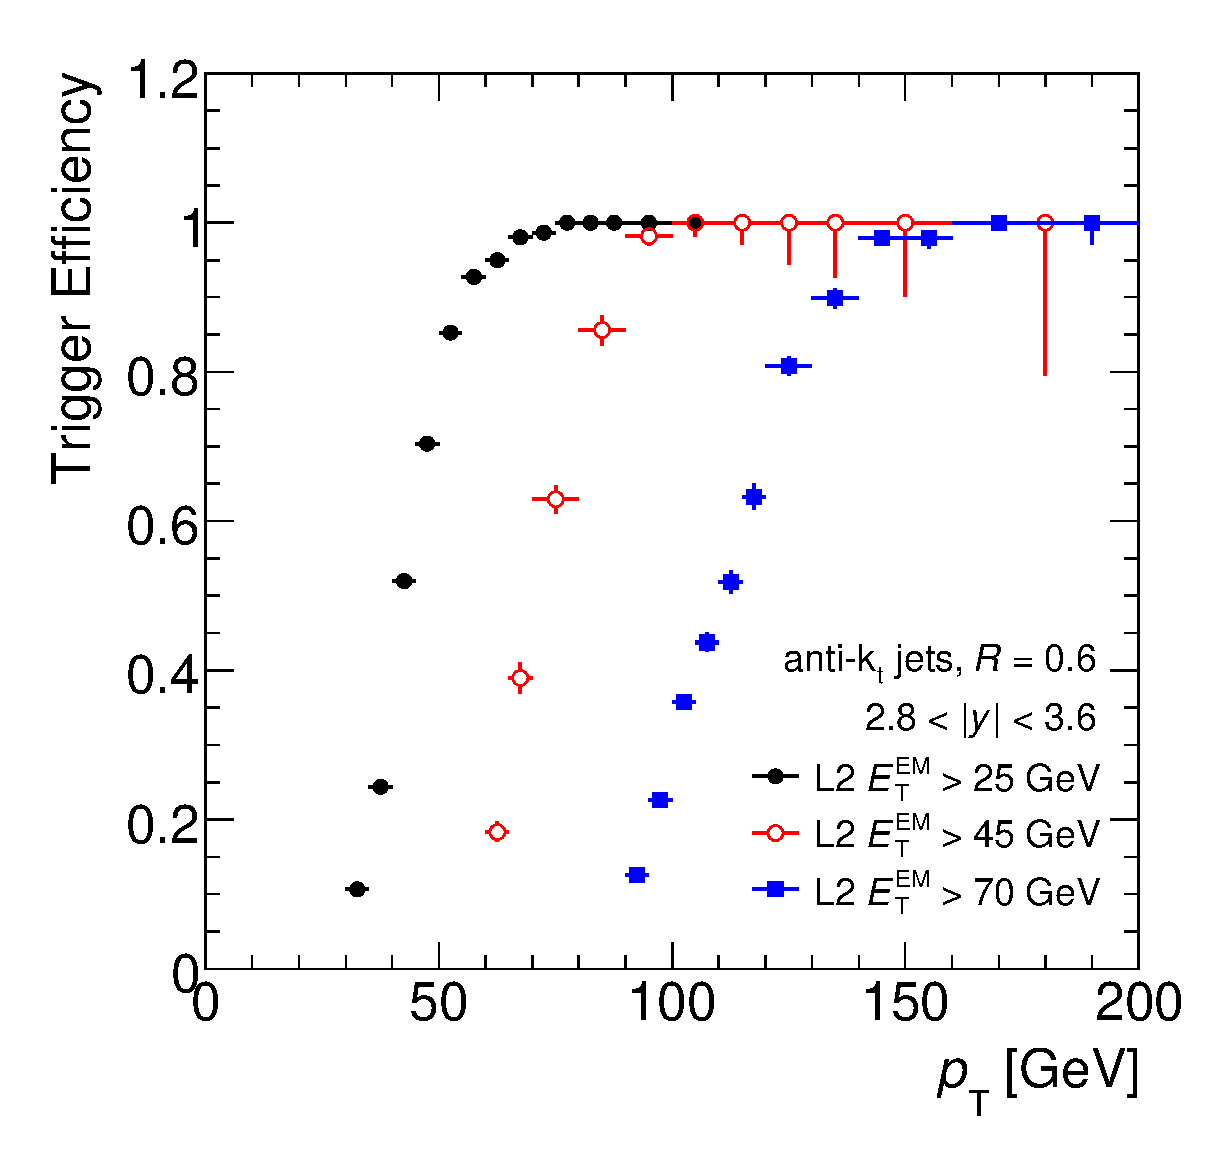
\includegraphics[width=\smallfigwidth]{chapters/forward-inclusive/transition_bin_triggers_L1L2_akt6.eps}
    \label{fig:forward-inclusive:transition_bin_triggers_L1L2_akt6}}
  \caption{Jet trigger efficiency in the HEC-FCAL transition region $2.8 \leq \absRap < 3.6$
           at L1 (top) and combined L1+L2 (bottom). Trigger efficiencies are presented
           as a function of reconstructed jet \pT for \akt jets with $R=0.4$ (left)
           and $R=0.6$ (right), shown for three trigger thresholds. The trigger
           thresholds are at the electromagnetic scale, while the jet \pT is at
           the calibrated scale (see \SectionRef{sec:analysis-tools:jet_reconstruction}).}
  \label{fig:forward-inclusive:transition_bin_trigger_efficiencies}
\end{figure}

\begin{table}
\begin{center}
  \begin{tabular}{ l @{\hspace{1cm}}l @{\hspace{1cm}}l }
  \pT range $[\GeV]$ & Period A--C & Period E5--F        \\
  \midrule
  20--30             & L1\_MBTS\_1 & n/a                 \\
  30--45             & L1\_MBTS\_1 & n/a                 \\
  45--60             & L1\_MBTS\_1 & n/a                 \\
  60--80             & n/a         & L1\_J10 or L1\_FJ10 \\
  80--110            & n/a         & L1\_J10 or L1\_FJ10 \\
  110--160           & n/a         & L1\_J30 or L1\_FJ30 \\
  160--210           & n/a         & L1\_J55 or L1\_FJ55 \\
  210--260           & n/a         & L1\_J55 or L1\_FJ55 \\
  260+               & n/a         & L1\_J55 or L1\_FJ55 \\
  \midrule
  \pT range $[\GeV]$ & \multicolumn{2}{l}{Period G--I}                           \\
  \midrule
  20--30             & \multicolumn{2}{l}{n/a}                                   \\
  30--45             & \multicolumn{2}{l}{n/a}                                   \\
  45--60             & \multicolumn{2}{l}{n/a}                                   \\
  60--80             & \multicolumn{2}{l}{n/a}                                   \\
  80--110            & \multicolumn{2}{l}{EF\_j30\_jetNoEF or EF\_fj30\_jetNoEF} \\
  110--160           & \multicolumn{2}{l}{EF\_j50\_jetNoEF or EF\_fj50\_jetNoEF} \\
  160--210           & \multicolumn{2}{l}{EF\_j50\_jetNoEF or EF\_fj50\_jetNoEF} \\
  210--260           & \multicolumn{2}{l}{EF\_j75\_jetNoEF or EF\_fj75\_jetNoEF} \\
  260+               & \multicolumn{2}{l}{EF\_j75\_jetNoEF or EF\_fj75\_jetNoEF} \\
  \end{tabular}
  \caption{The trigger chains used for the inclusive jet analysis in the transition
           region, $2.8 \leq \absRap < 3.6$. The first four periods (A--D) could not
           be used, as the forward jet trigger had not yet been commissioned, while
           additional problems made it unreliable for subperiods E1--4. L1\_MBTS\_1
           was found to be fully efficient for transition jets and hence was used
           in early periods to trigger low \pT jets here.}
  \label{tab:forward-inclusive:TriggersTransition}
\end{center}
\end{table}

\TableRef{tab:forward-inclusive:trigger-explanation} provides a series of example
trigger decisions for jets in or around the transition region, according to their
\pT and which triggers are passed. For the sake of this example, all of these imaginary
events are considered to belong to period F.

\begin{table}
\begin{center}
  \begin{tabular}{ c c c c c c }
    Period & Jet \absRap & Jet \pT $[\GeV]$ & L1\_J10 & L1\_FJ10 & Event accepted? \\
    \midrule
    F      & 3.0         & 30               & passed  & passed   & no              \\
    F      & 3.0         & 70               & passed  & passed   & yes             \\
    F      & 3.0         & 70               & failed  & passed   & yes             \\
    F      & 3.0         & 70               & passed  & failed   & yes             \\
    F      & 2.6         & 70               & failed  & passed   & no              \\
    F      & 3.8         & 70               & failed  & passed   & yes             \\
  \end{tabular}
  \caption{Sample table demonstrating trigger decisions and event acceptance for
           a series of possible jets in period F.}
  \label{tab:forward-inclusive:trigger-explanation}
\end{center}
\end{table}

To avoid double counting in taking the OR of central and forward chains, these events
have to be considered separately with respect to those only passing a central or
a forward threshold.

Consider the set of all events which pass the OR of the central and forward chain,
in other words, those which are taken by either the central trigger, forward trigger
or both at once. In these events, which are already triggered and accepted, it is
possible to examine the complete set trigger information; in particular it can be
determined which triggers each of these events would have passed \textit{before prescale was applied}.

Triggered jets in the transition bin can therefore be divided into three classes, according to
whether they would have passed, before prescale, the central threshold, the forward threshold or
both. For each of these classes, an equivalent luminosity is calculated, summing over all luminosity
blocks. The luminosity for jets selected by the central trigger is given by

\begin{equation}
  \mathcal{L}_{\mathrm{J}} = \sum_{\mathrm{LB}} \frac{\mathcal{L}_{\mathrm{LB}}}{P^{\mathrm{J}}_{\mathrm{LB}}}
\end{equation}

\noindent where $P^{\mathrm{J}}_{\mathrm{LB}}$ is the prescale of the central trigger for each luminosity
block, and $\mathcal{L}_{\mathrm{LB}}$ its luminosity; for jets selected by the forward
trigger the equivalent luminosity will be

\begin{equation}
  \mathcal{L}_{\mathrm{FJ}} = \sum_{\mathrm{LB}} \frac{\mathcal{L}_{\mathrm{LB}}}{P^{\mathrm{FJ}}_{\mathrm{LB}}}
\end{equation}

Finally, for events taken, before prescale, by both central and forward trigger, the
equivalent luminosity is

\begin{equation}
  \mathcal{L}_{\mathrm{JFJ}} = \sum_{\mathrm{LB}} \frac{\mathcal{L}_{\mathrm{LB}}}{P^{\mathrm{J}}_{\mathrm{LB}} P^{\mathrm{FJ}}_{\mathrm{LB}}/(P^{\mathrm{J}}_{\mathrm{LB}} + P^{\mathrm{FJ}}_{\mathrm{LB}}-1)}
  \label{eq:forward-inclusive:final_luminosity}
\end{equation}

Let $N_{\mathrm{J}}$, $N_{\mathrm{FJ}}$ and $N_{\mathrm{JFJ}}$ denote respectively the number of events taken,
by the central trigger, by the forward trigger, and by both triggers. The \xs, before
any other correction, is then given by

\begin{equation}
 \sigma = \frac{N_{\mathrm{J}}}{\mathcal{L}_{\mathrm{J}}} + \frac{N_{\mathrm{FJ}}}{\mathcal{L}_{\mathrm{FJ}}} + \frac{N_{\mathrm{JFJ}}}{\mathcal{L}_{\mathrm{JFJ}}}
\end{equation}

\noindent ensuring that events passing two triggers are properly treated in a separate
category and not double-counted.

\subsection{Trigger Efficiencies}
\label{sec:forward-inclusive:trigger_efficiencies}
In general, the trigger strategy has been designed to ensure that all jets are on
the 99\% plateau; however, due to a known problem with a dead trigger tower in a
region of the FCAL, the efficiency of some forward jet triggers reaches a plateau
at less than 100\%.

The effects of these inefficiencies are small, less than 5\%, which is helped by
the fact that a per-event efficiency definition is used, so that an offline jet
falling into a lower efficiency region can still be accepted if there is another
jet in the event. Accordingly, a systematic uncertainty is applied rather than restricting
the phase-space of the measurement. \FigureRef{fig:detector:forward_bin_trigger_efficiencies}
shows the trigger efficiency in the most forward rapidity region, $3.6 \leq \absRap < 4.4$,
where the jets are fully contained by the FCAL. Irregularities in the trigger
plateau arising from the problematic trigger tower can be seen here.

\section{Unfolding Detector Effects}
\label{sec:forward-inclusive:unfolding}
Detector inefficiencies and resolutions, apart from those corrected for in by
the jet calibration scheme, are corrected for using an iterative unfolding
method: the IDS scheme detailed in \SectionRef{sec:analysis-tools:unfolding}.
The same binning is used as for the final distributions and the unfolding is
performed separately for each rapidity bin.

A detector level \xs is constructed in each case, by combining the set of events
passing each trigger and correcting, in each case, for the appropriate integrated luminosity by
that trigger. This detector level \xs is then used as the input for the unfolding
procedure.

The effect of any potential mismodelling of the \xs shape in \MC is examined by
comparing the shapes of detector level spectra in \MC and in data. These are
used to derive an event-by-event reweighting function that is applied to the
\MC particle level spectra, in each bin of \rap and \pT, before the unfolding factors are calculated.
\FigureRef{fig:forward-inclusive:data_mc_control_distributions} shows the level of agreement
between \Pythia and the data for two sample distributions.

\begin{figure}[htpb]
  \subfloat[Data to \MC comparison for \akt $R=0.4$ jets, in the region $2.1 \leq \rap < 2.8$]{
    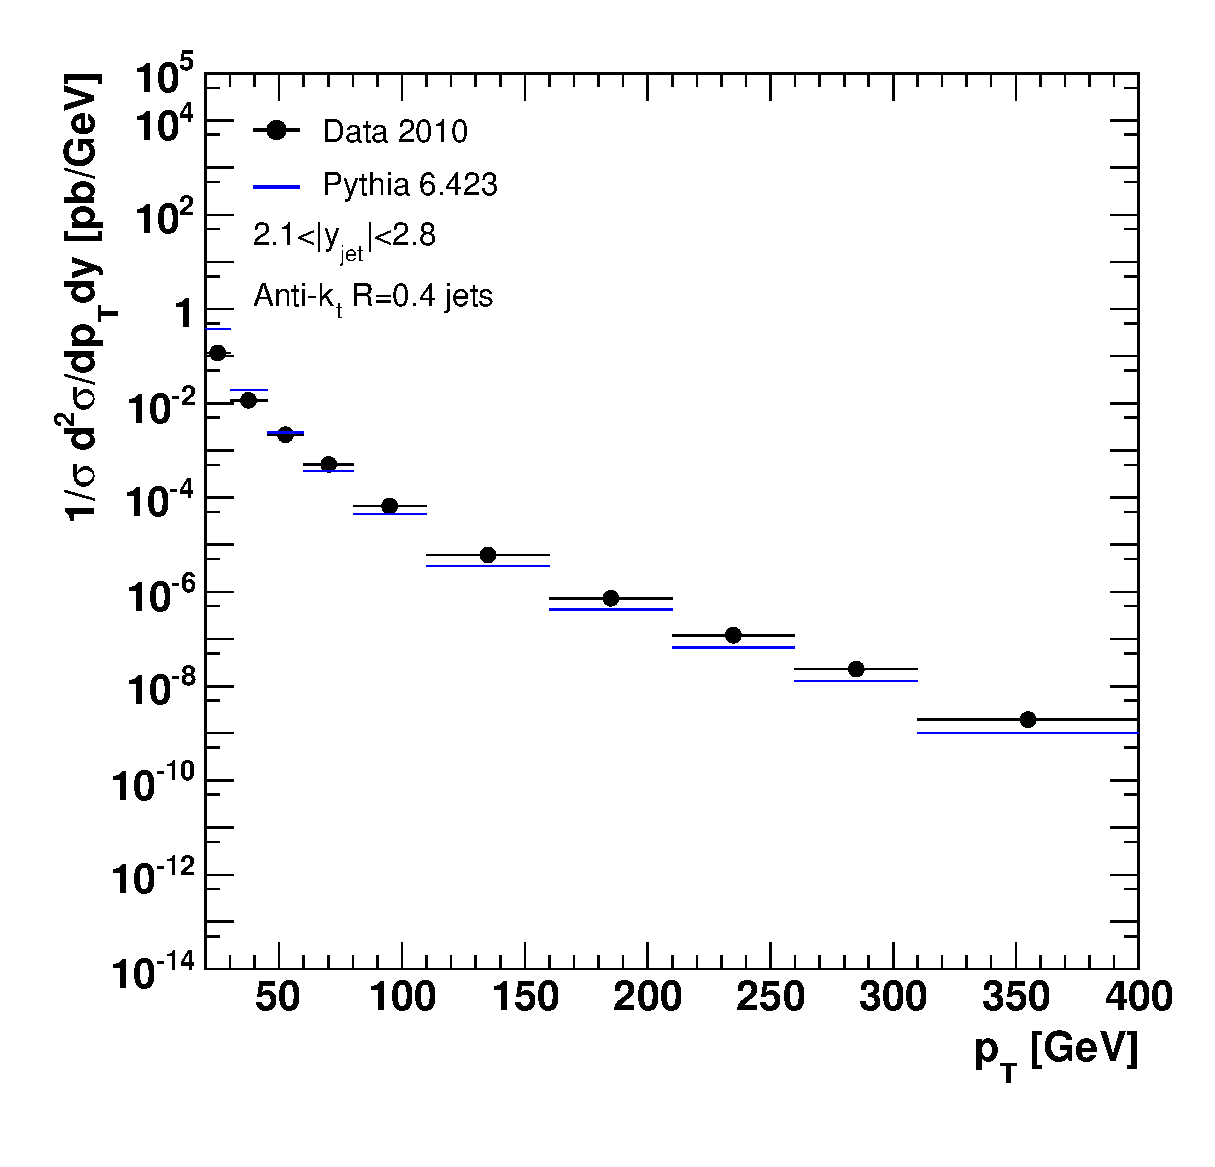
\includegraphics[width=\smallfigwidth]{chapters/forward-inclusive/Control.AntiKt4.2.1y2.8.eps}
    \label{fig:forward-inclusive:akt4_control}}
  \quad
  \subfloat[Data to \MC comparison for \akt $R=0.6$ jets, in the region $3.6 \leq \rap < 4.4$]{
    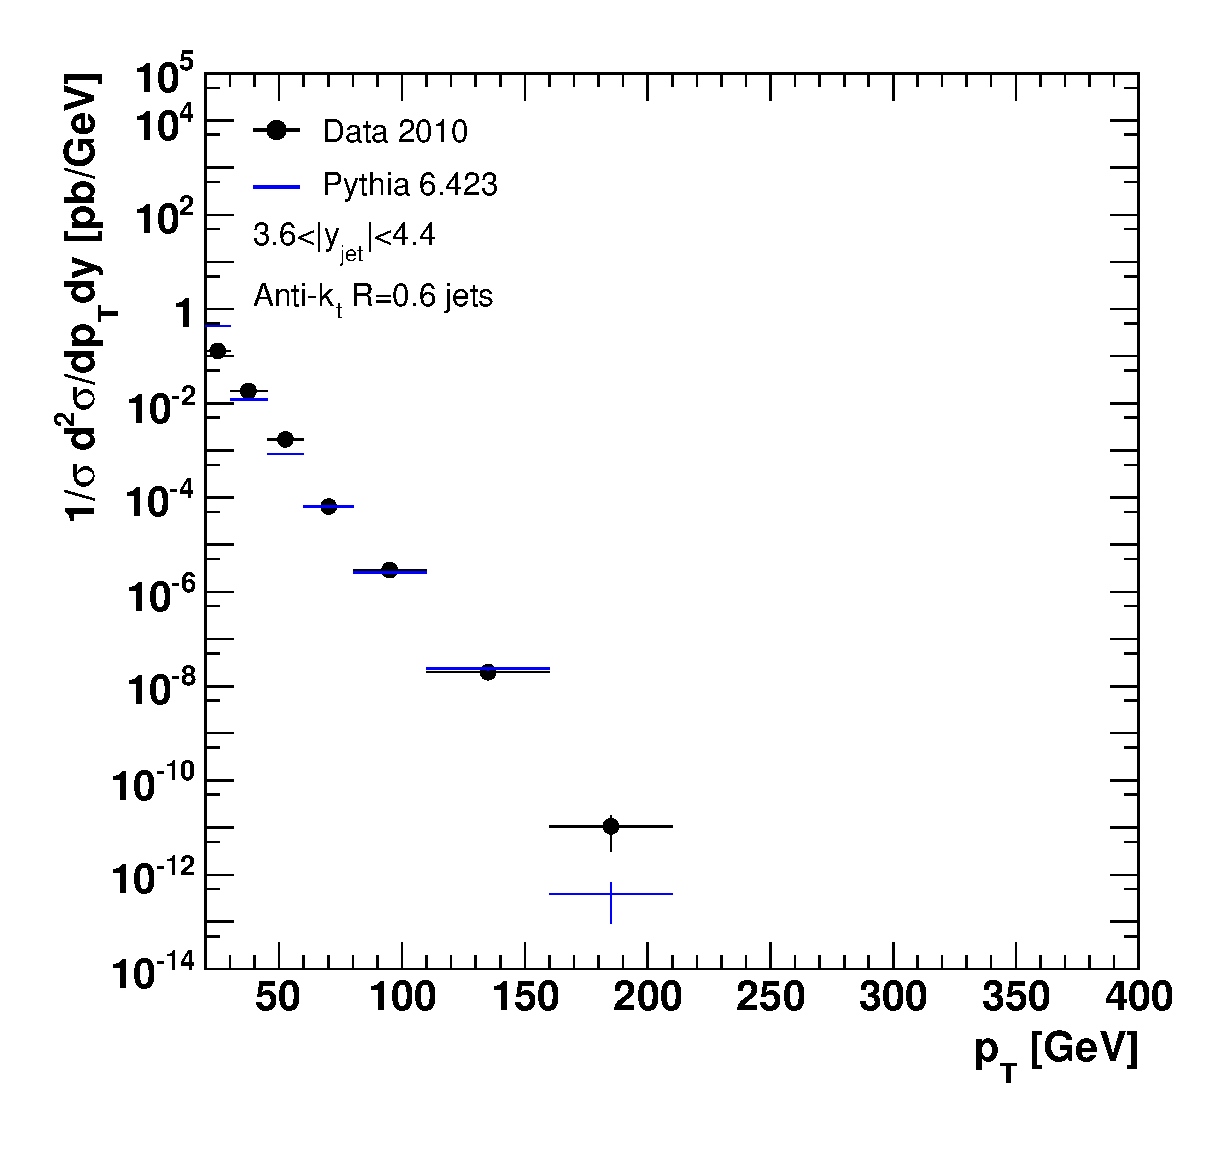
\includegraphics[width=\smallfigwidth]{chapters/forward-inclusive/Control.AntiKt6.3.6y4.4.eps}
    \label{fig:forward-inclusive:akt6_control}}
  \caption{Control distributions, used to demonstrate the level of agreement between data and \MC; data is shown in black, with \Pythia in blue. \protect\subref{fig:forward-inclusive:akt4_control} shows the comparison for \akt $R=0.4$ jets in the region $2.1 \leq \rap < 2.8$, while \protect\subref{fig:forward-inclusive:akt6_control} shows the comparison for \akt $R=0.6$ jets in the region $3.6 \leq \rap < 4.4$.}
  \label{fig:forward-inclusive:data_mc_control_distributions}
\end{figure}

\section{Systematic Uncertainties}
\label{sec:forward-inclusive:systematics}
Track jets, reconstructed using only information from the tracking detector, are
used to provide an in-situ estimate of jet reconstruction efficiency. The
frequency with which a calorimeter jet was reconstructed, given the existence of
a nearby track jet, was studied in data and \MC and used to infer an uncertainty
on the calorimeter jet reconstruction efficiency measured in \MC. This
disagreement of 1\%, or 2\% for the lowest \pT jets, was taken as a systematic
uncertainty.

The jet energy scale uncertainty, evaluated as described in \SectionRef{sec:analysis-tools:jes_uncertainty},
is the largest single contributor to systematic uncertainties due to the steeply
falling \xs as a function of jet \pT. The JES uncertainty was treated in the same way
as energy resolution, measured from \dijet balancing in data, and
angular resolution, estimated in \MC by matching particle level and detector level
jets; each of these quantities was varied up and down by one standard deviation
and the relative per-bin shift in jet yield was taken as a systematic
uncertainty for that bin. In the central region, $\absRap < 0.8$, the
uncertainty is lower than 4.6\% for all jets with $\pT \geq \unit{20}{\GeV}$, while
for jets with $60 \leq \pT < \unit{800}{\GeV}$ the uncertainty is below 2.5\%, as
can be seen from \FigureRef{fig:analysis-tools:JESUncertainty}.

By propagating these uncertainties through the unfolding procedure, an estimate
of the systematic uncertainty due to unfolding can also be obtained. This is
approximately 5\% at low and high \pT and smaller at intermediate \pT values.
An additional uncertainty of 3.4\% comes from the luminosity measurement.

\begin{figure}[htpb]
  \subfloat[\Akt $R=0.4$ jets, $\absRap < 0.3$]{
    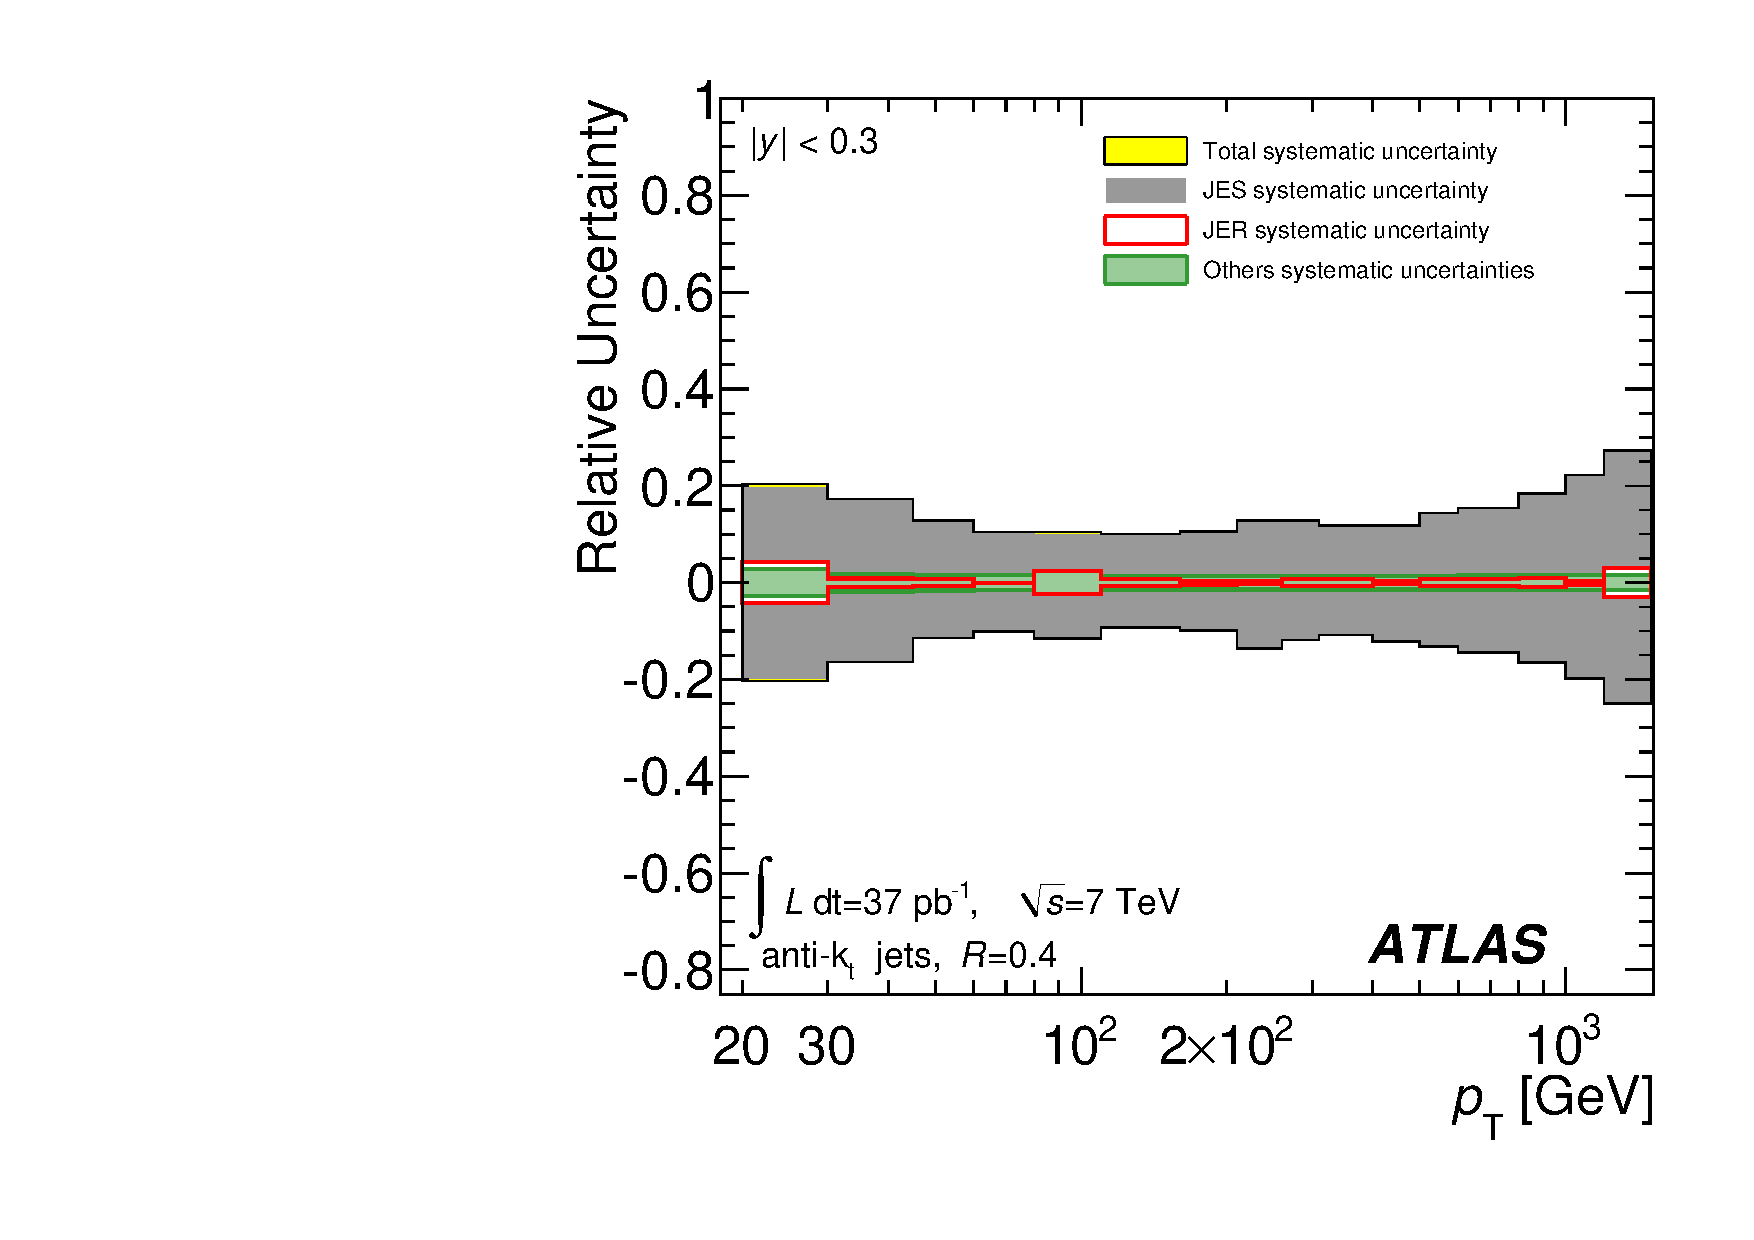
\includegraphics[width=\smallfigwidth]{chapters/forward-inclusive/InclusivePtSysIDS_AntiKt04_00_03.pdf}
    \label{fig:forward-inclusive:uncertainties_akt4}}
  \quad
  \subfloat[\Akt $R=0.6$ jets, $0.8 \leq \absRap < 1.2$]{
    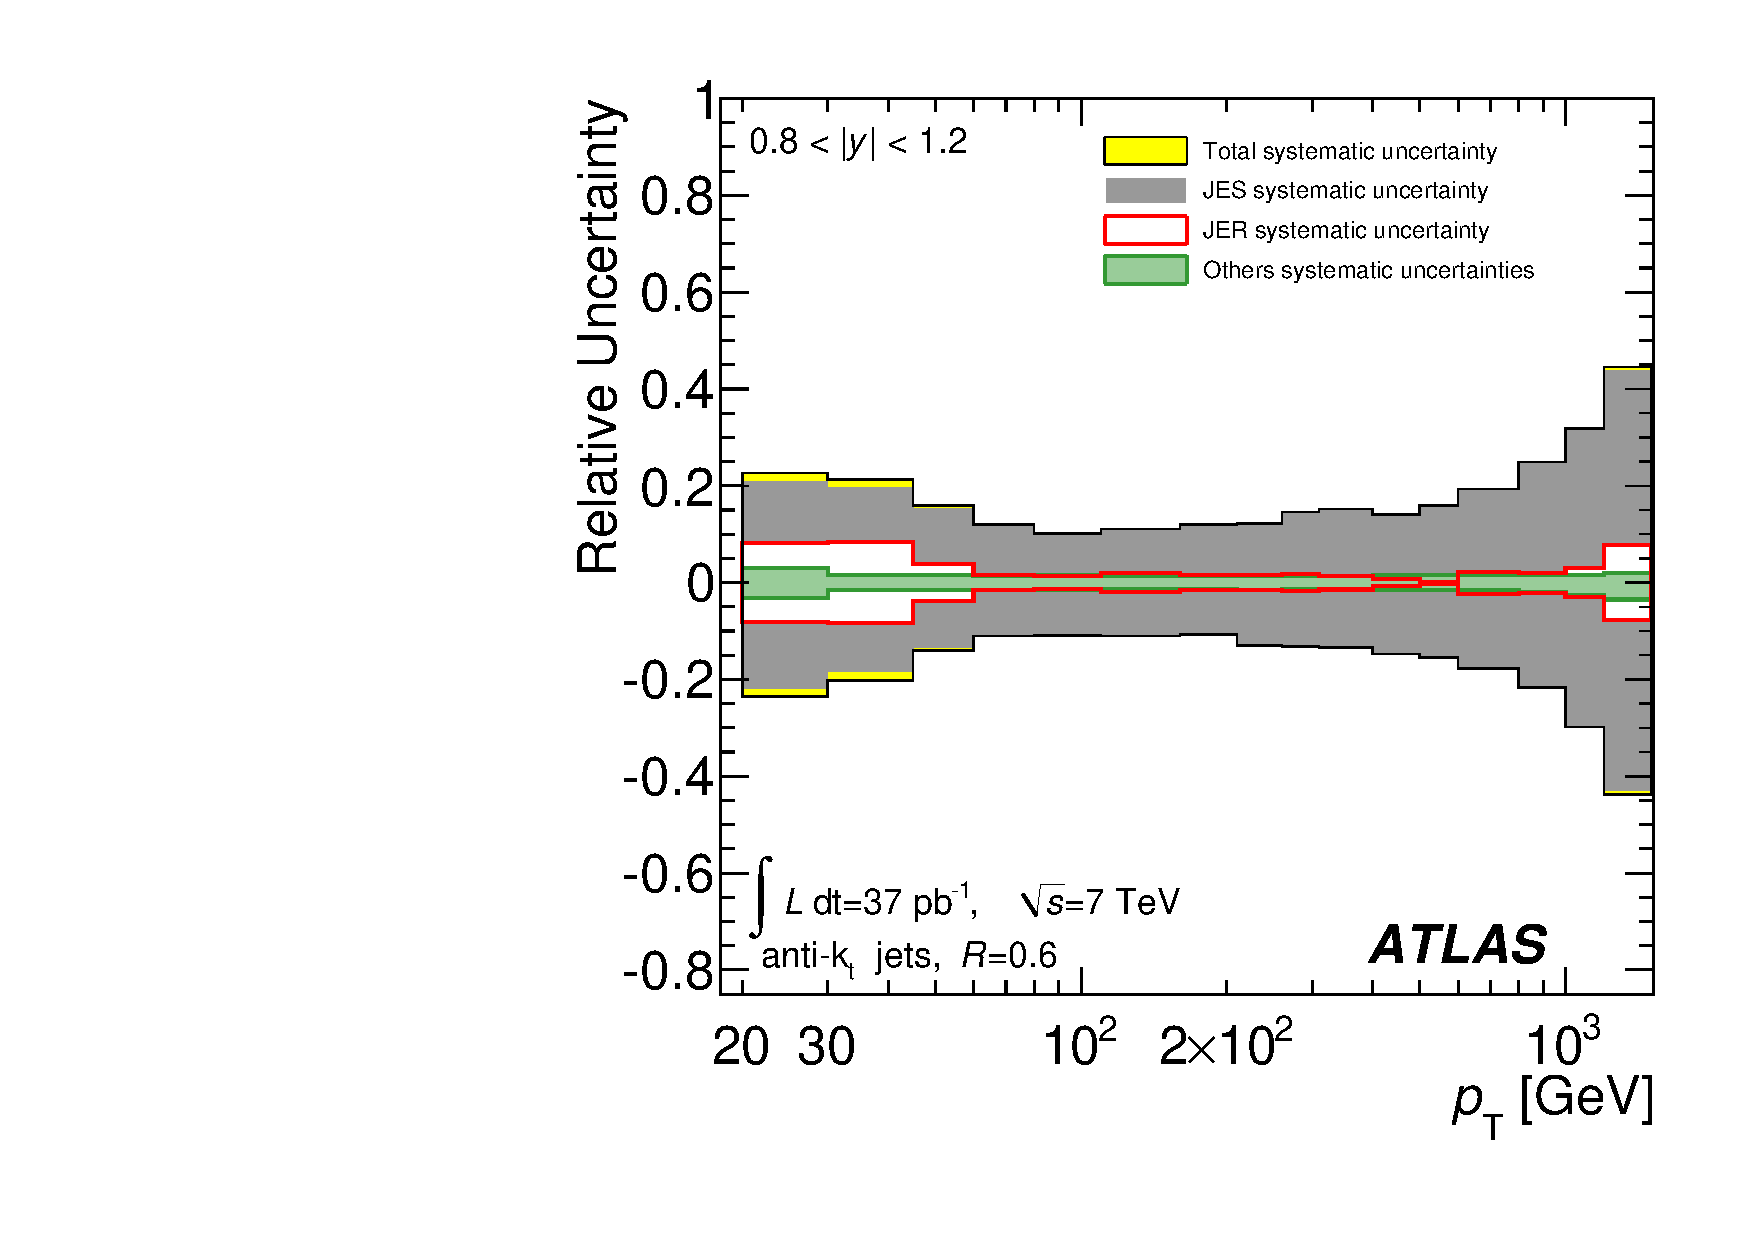
\includegraphics[width=\smallfigwidth]{chapters/forward-inclusive/InclusivePtSysIDS_AntiKt06_08_12.pdf}
    \label{fig:forward-inclusive:uncertainties_akt6}}
  \caption{Summary of relative systematic effects affecting the inclusive jets \xs. \protect\subref{fig:forward-inclusive:uncertainties_akt4} shows the uncertainty for \akt $R=0.4$ jets in the region $\absRap < 0.3$ while \protect\subref{fig:forward-inclusive:uncertainties_akt6} shows the corresponding uncertainty for \akt $R=0.6$ jets in the region $0.8 \leq \absRap < 1.2$. The jet energy scale uncertainty provides the dominant systematic in both cases.}
  \label{fig:forward-inclusive:uncertainties}
\end{figure}

Systematic uncertainties on the final \xs are obtained by summing all
uncertainties in quadrature to give a total uncertainty on the unfolded data; an
example of this process for two \absRap bins can be seen in \FigureRef{fig:forward-inclusive:uncertainties}.
However, the steeply falling jet \pT spectrum, especially at large rapidity,
unavoidably converts even small uncertainties in \pT into large errors on the
measured \xs.

\section{Theoretical Predictions}
\label{sec:forward-inclusive:theory_predictions}
The measured inclusive jet \xs{s} are compared to both NLO \pQCD predictions,
with corrections for non-perturbative effects, and to NLO \MC.

\subsection{Next-to-Leading Order Perturbative \QCD Calculations}
\label{sec:forward-inclusive:NLOpQCD}
Next-to-leading order (NLO) perturbative \QCD (\pQCD) predictions are produced using the \NLOjetpp 4.1.2~\cite{Nagy:2003:NLOjet}
program together with the CT10~\cite{Lai:2010:LHAPDF_CT10} NLO PDFs. The main uncertainties
on the NLO prediction come from the uncertainties on the PDFs, the choice of factorisation
and renormalisation scales (as discussed in \SectionRef{sec:bg-theory:qcd_factorisation})
and the uncertainty in the value of the strong coupling constant, \alphaS.

To estimate the uncertainty on the NLO prediction due to neglected higher-order
terms, each observable was recalculated while varying the renormalisation scale
by a factor of two with respect to the default choice, defined to be the \pT of
the hardest jet in the event. Similarly, to estimate the sensitivity to the choice
of scale where the PDF evolution is separated from the matrix element, the factorisation
scale was separately varied by a factor of two. The experimental uncertainties which
propagate through the PDF fits, together with the associated uncertainties on the
value of $\alphaS(M_Z)$ were used to determine uncertainty bands on the theoretical
predictions; a summary of these corrections can be seen in \FigureRef{fig:forward-inclusive:theory_uncertainties}.
Uncertainties due to the choice of PDF were evaluated by creating predictions using
four different PDF sets and presenting each of these on the final plots.
%The uncertainties due to the choice
%of PDF were evaluated by repeating this calculation using four additional PDFs,
%with the uncertainty on the value of $\alphaS(M_Z)$ established in the same way.
%A summary of these corrections for two sample PDFs can be seen in \FigureRef{fig:forward-inclusive:theory_uncertainties}.

\begin{figure}[htpb]
  \subfloat[\Akt $R=0.4$ jets, $\absRap < 0.3$]{
    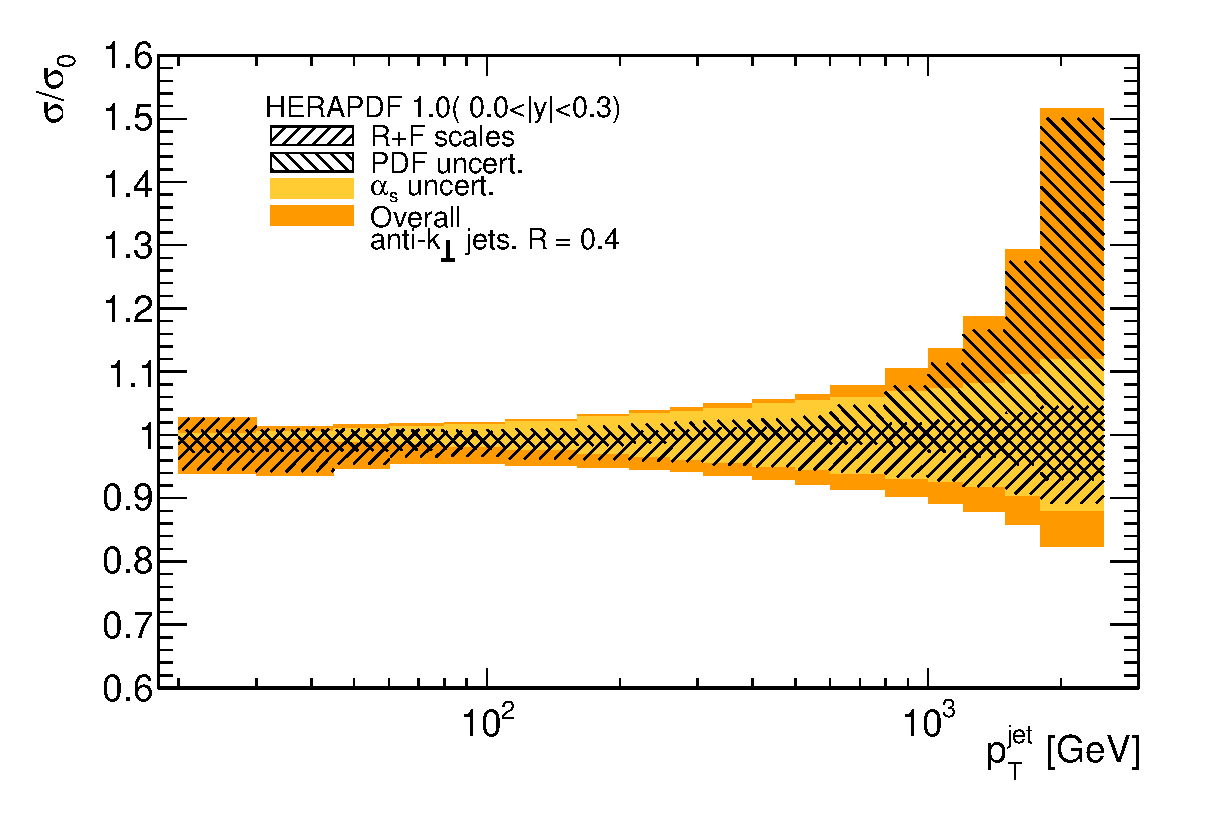
\includegraphics[width=\smallfigwidth]{chapters/forward-inclusive/bands_InclJets04_00_03_HERAPDF10_EIG.eps}
    \label{fig:forward-inclusive:theory_uncertainties_akt4}}
  \quad
  \subfloat[\Akt $R=0.6$ jets, $\absRap < 1.2$]{
    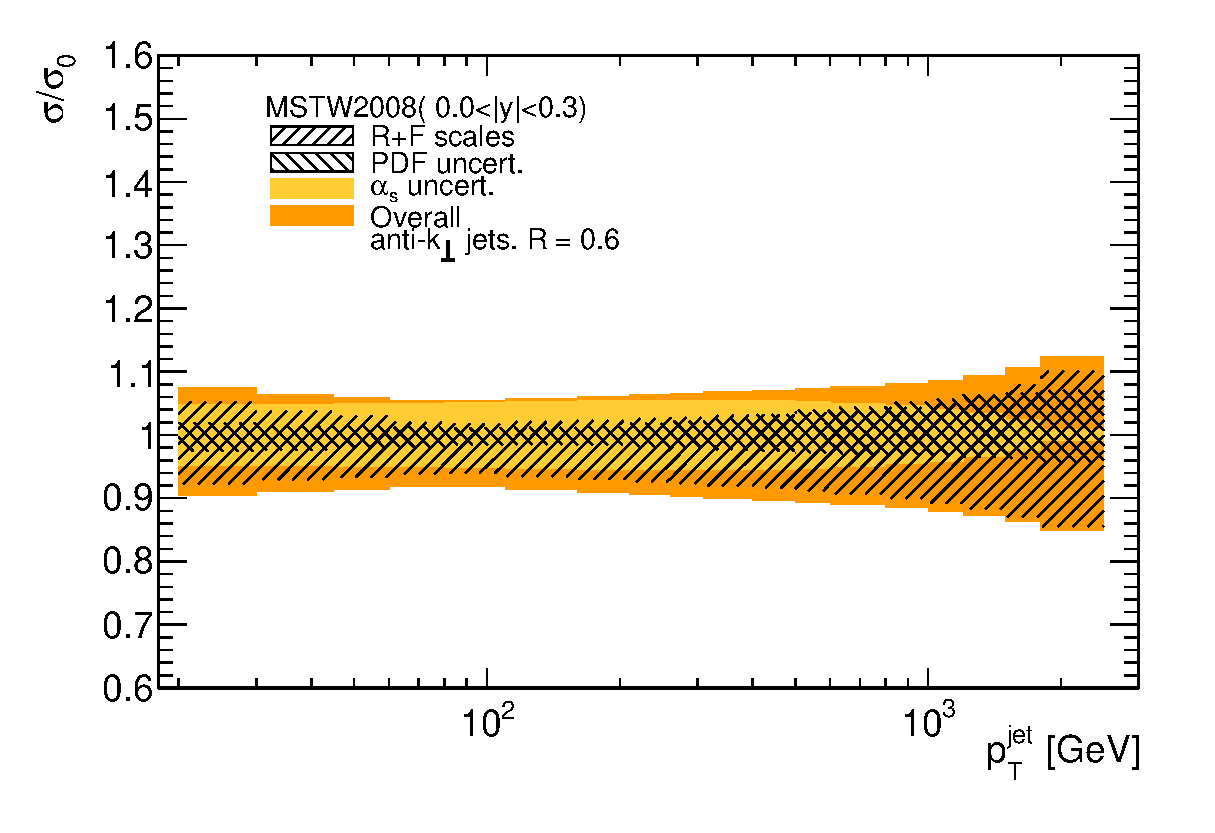
\includegraphics[width=\smallfigwidth]{chapters/forward-inclusive/bands_InclJets06_00_03_MSTW2008nlo90cl.eps}
    \label{fig:forward-inclusive:theory_uncertainties_akt6}}
  \caption{Summary of theory uncertainties arising from the scale choice, uncertainties inherent to the chosen PDF and uncertainties arising from the value of \alphaS. \protect\subref{fig:forward-inclusive:theory_uncertainties_akt4} shows the ratio of the \xs to the nominal \xs for HERAPDF, using \akt $R=0.4$ jets in the region $\absRap < 0.3$ while \protect\subref{fig:forward-inclusive:theory_uncertainties_akt6} shows the same quantity for MSTW2008, using \akt $R=0.6$ jets in the region $\absRap < 0.3$.}
  \label{fig:forward-inclusive:theory_uncertainties}
\end{figure}

Parton level \xs{s}, obtained from fixed-order NLO calculations must be
corrected for non-perturbative effects before they can be compared with data. This
is done by using leading-logarithmic parton shower generators (in this case, \Pythia
with the AUET2B CTEQ6L1 tune~\cite{Pumplin:2002:CTEQ6L1}) to evaluate the ratio of \xs{s} with and without
hadronisation and underlying event. The parton level \xs{s} are then multiplied,
bin-by-bin, by this ratio; tacitly assuming that the effects of soft and hard physics can be
factorised. The uncertainty is estimated as the maximum spread of the correction
factors obtained from performing this procedure using different \Pythia tunes.

\subsection{Next-to-leading Order \MC with Parton Shower}
The \Powheg generator (see \SectionRef{sec:bg-theory:MC:Powheg}) is used to provide
an NLO matrix element prediction. The use of an event generator with NLO matrix elements,
including the simulation of the parton shower, the hadronisation, and the underlying
event, creates a more coherent theoretical prediction and overcomes the need for
separate non-perturbative corrections.

\section{Inclusive Jet \Xs{s}}
The double-differential inclusive jet \xs is shown in \FigureRef{fig:forward-inclusive:InclusiveCrossSectionAKT4}
and \FigureRef{fig:forward-inclusive:InclusiveCrossSectionAKT6} for jets reconstructed
using the \akt algorithm with $R=0.4$ and $R=0.6$ respectively. The measurement
covers the jet \pT range from \unit{20}{\GeV} to \unit{1.5}{\TeV}: spanning two orders
of magnitude in \pT and seven orders of magnitude in \xs. Statistical and
systematic errors on the data are shown, as discussed in \SectionRef{sec:forward-inclusive:systematics},
and the unfolded data is compared to NLO \pQCD predictions which are corrected
for non-perturbative effects as discussed in \SectionRef{sec:forward-inclusive:NLOpQCD}.
It can be seen from \FigureRef{fig:forward-inclusive:NLORatio} that the data and
the theory predictions are generally in good agreement within the experimental and
theoretical uncertainties, with some minor differences visible at high jet \pT and
\absRap.

\begin{figure}
  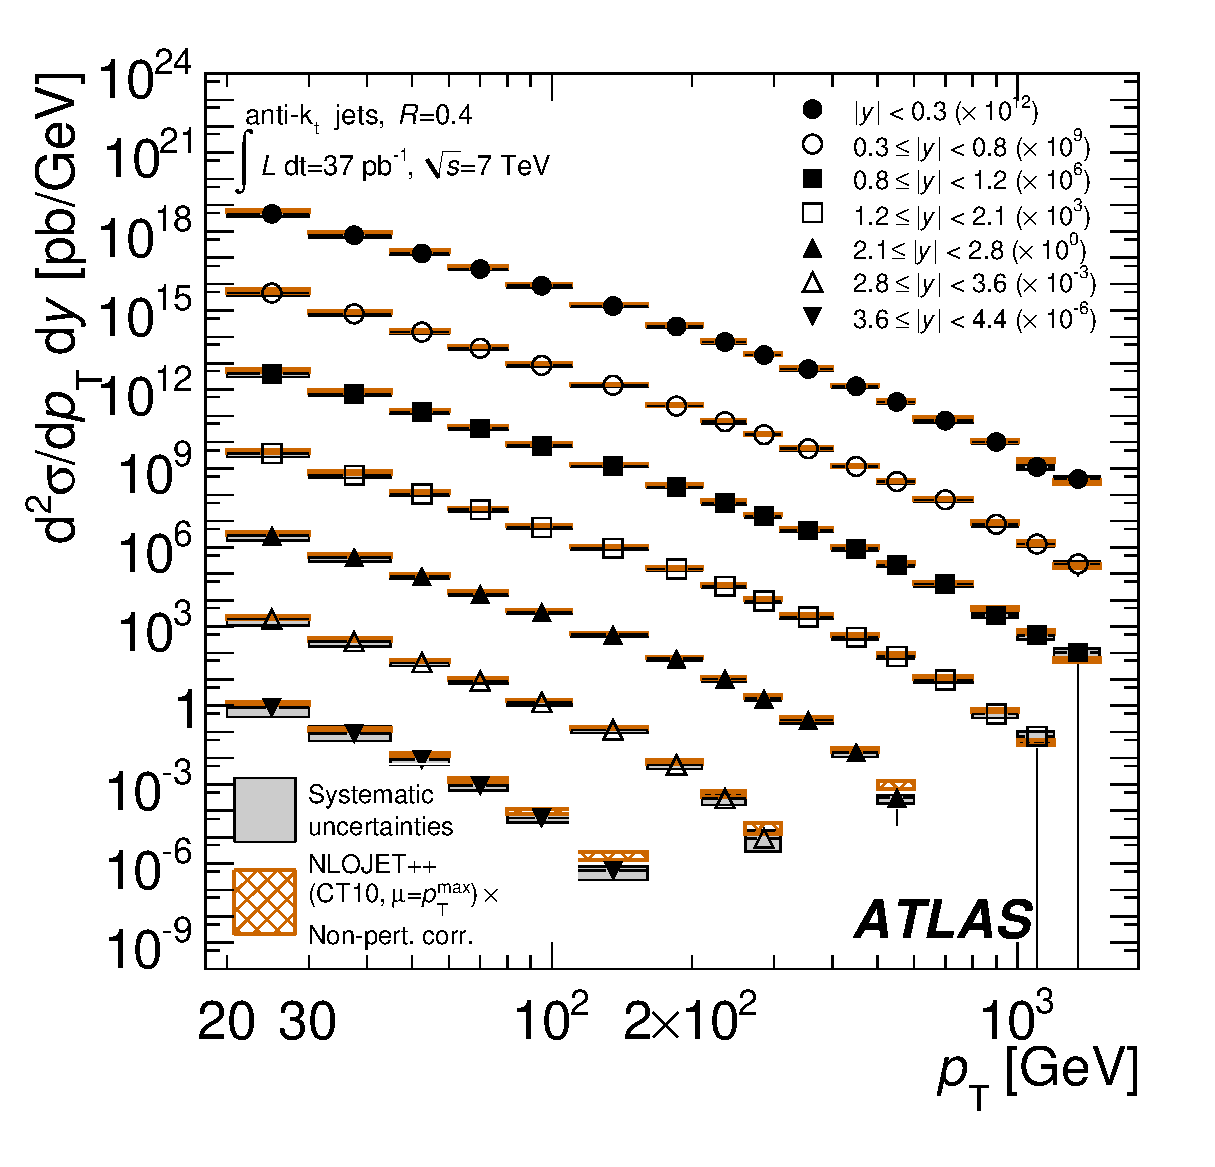
\includegraphics[width=\largefigwidth]{chapters/forward-inclusive/InclusivePtIDS_CT10_AntiKt04.eps}
  \caption{Inclusive jet double-differential \xs as a function of jet \pT in
     different regions of \absRap for jets identified using the \akt algorithm with
     $R=0.4$. For convenience, the \xs{s} are multiplied by the factors indicated
     in the legend. The data are compared to NLO \pQCD calculations to which non-perturbative
     corrections have been applied. The error bars indicate the statistical uncertainty
     on the measurement, and the dark-shaded band indicates the quadratic sum of the
     experimental systematic uncertainties, dominated by the jet energy scale uncertainty.
     There is an additional overall uncertainty of 3.4\% due to the luminosity measurement
     that is not shown. The theory uncertainty (light cross-hatched band) shown is the quadratic
     sum of uncertainties from the choice of renormalisation and factorisation scales,
     parton distribution functions, \alphaS($M_Z$), and the modelling of non-perturbative
     effects, as described in the text.}
  \label{fig:forward-inclusive:InclusiveCrossSectionAKT4}
\end{figure}

\begin{figure}
  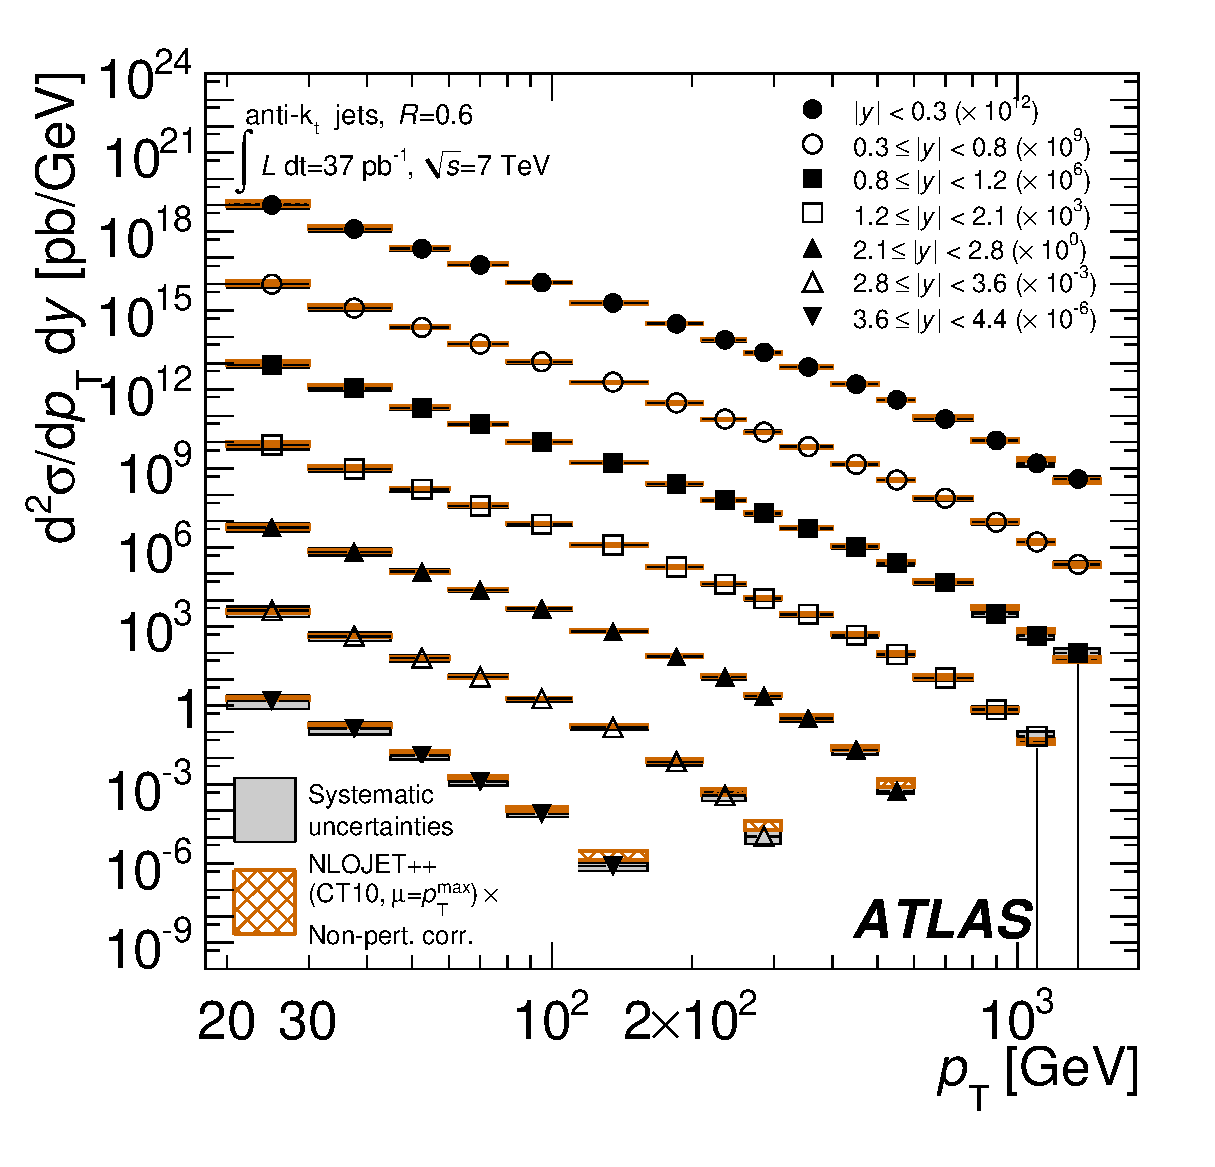
\includegraphics[width=\largefigwidth]{chapters/forward-inclusive/InclusivePtIDS_CT10_AntiKt06.eps}
  \caption{Inclusive jet double-differential \xs as a function of jet \pT in
    different regions of \absRap for jets identified using the \akt algorithm with
    $R=0.6$. For convenience, the \xs{s} are multiplied by the factors indicated
    in the legend. The data are compared to NLO \pQCD calculations to which non-perturbative
    corrections have been applied. The theoretical and experimental uncertainties
    indicated are calculated as described in \FigureRef{fig:forward-inclusive:InclusiveCrossSectionAKT4}.}
  \label{fig:forward-inclusive:InclusiveCrossSectionAKT6}
\end{figure}

\begin{figure}[htpb]
  \subfloat[\Akt $R=0.4$ jets, central rapidities]{
    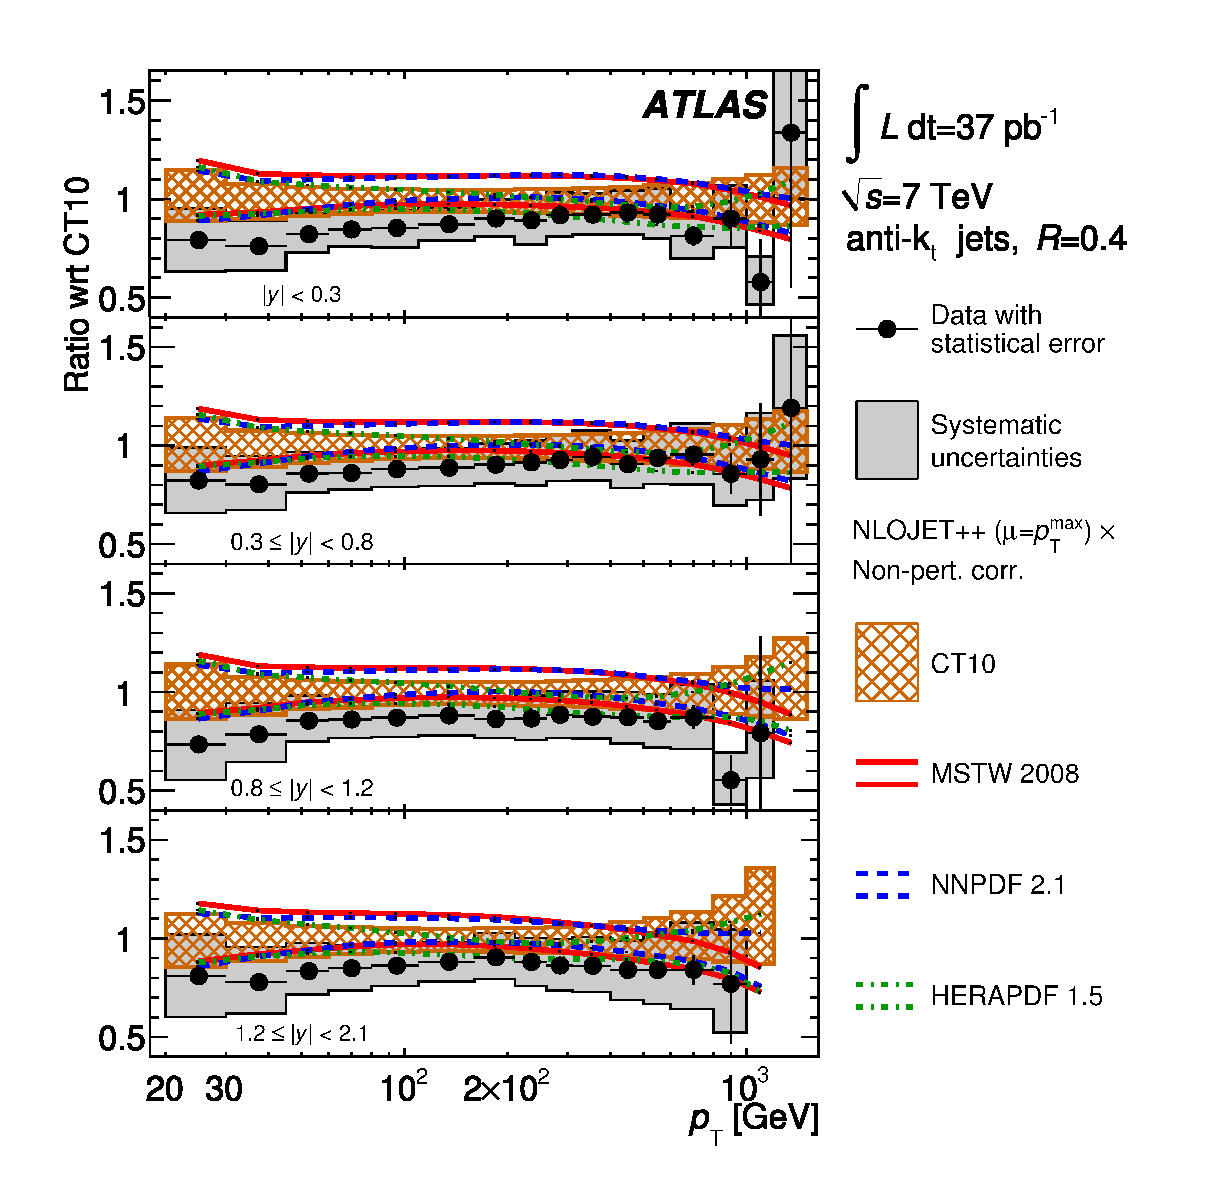
\includegraphics[width=\smallfigwidth]{chapters/forward-inclusive/InclusivePtIDSRatioCentral_CT10_AntiKt04.eps}
    \label{fig:forward-inclusive:NLORatioCentral_akt4}}
  \quad
  \subfloat[\Akt $R=0.6$ jets, central rapidities]{
    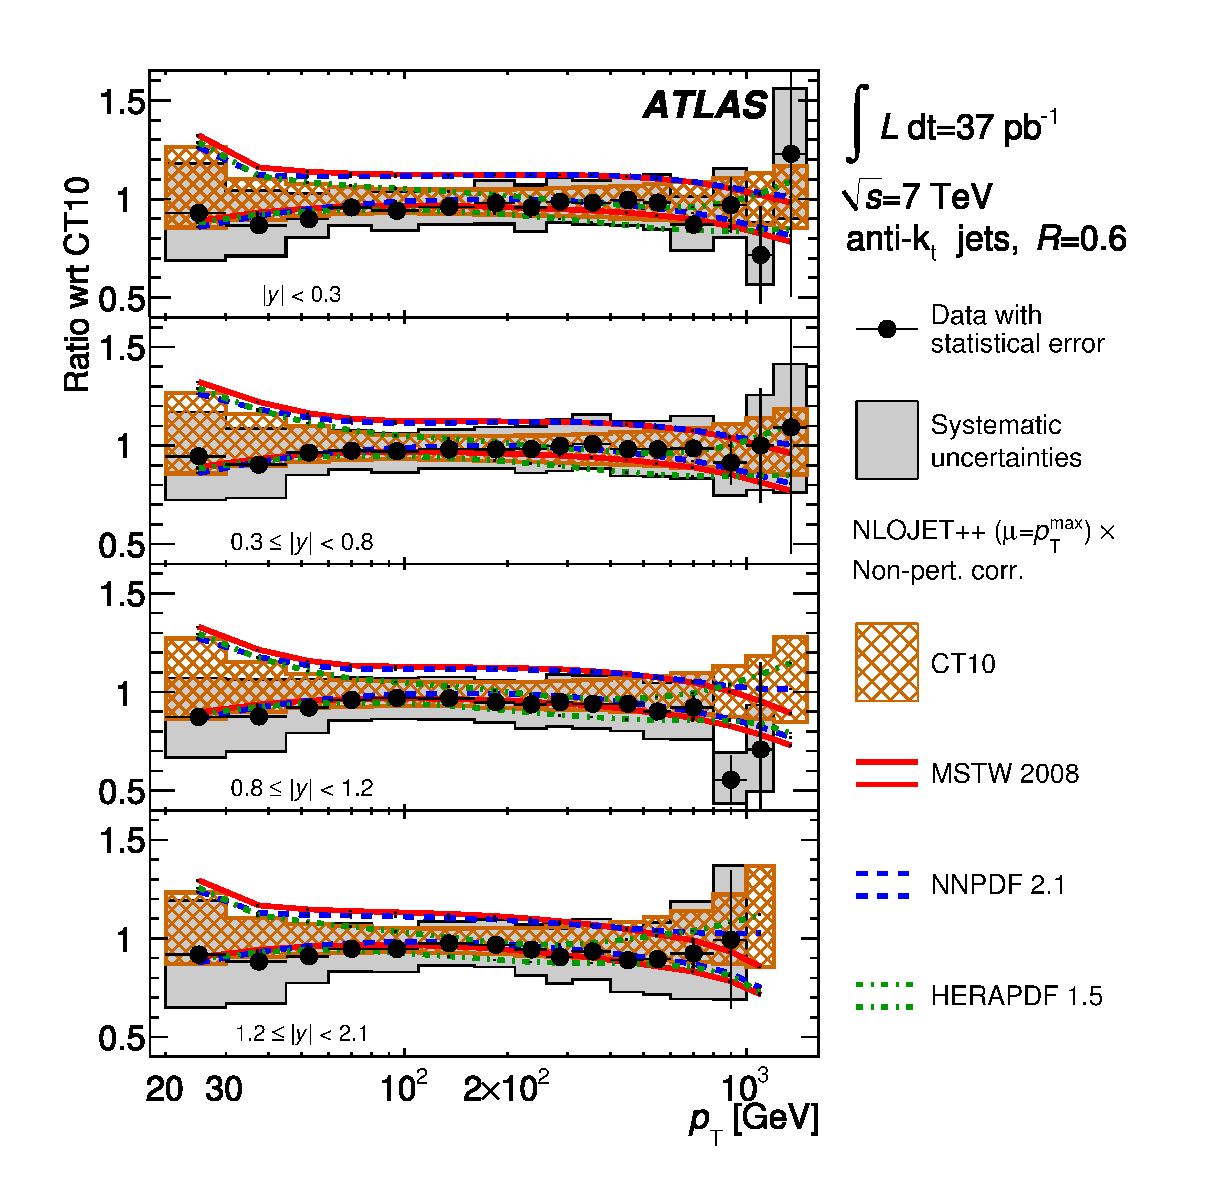
\includegraphics[width=\smallfigwidth]{chapters/forward-inclusive/InclusivePtIDSRatioCentral_CT10_AntiKt06.eps}
    \label{fig:forward-inclusive:NLORatioCentral_akt6}}
  \\
  \subfloat[\Akt $R=0.4$ jets, forward rapidities]{
    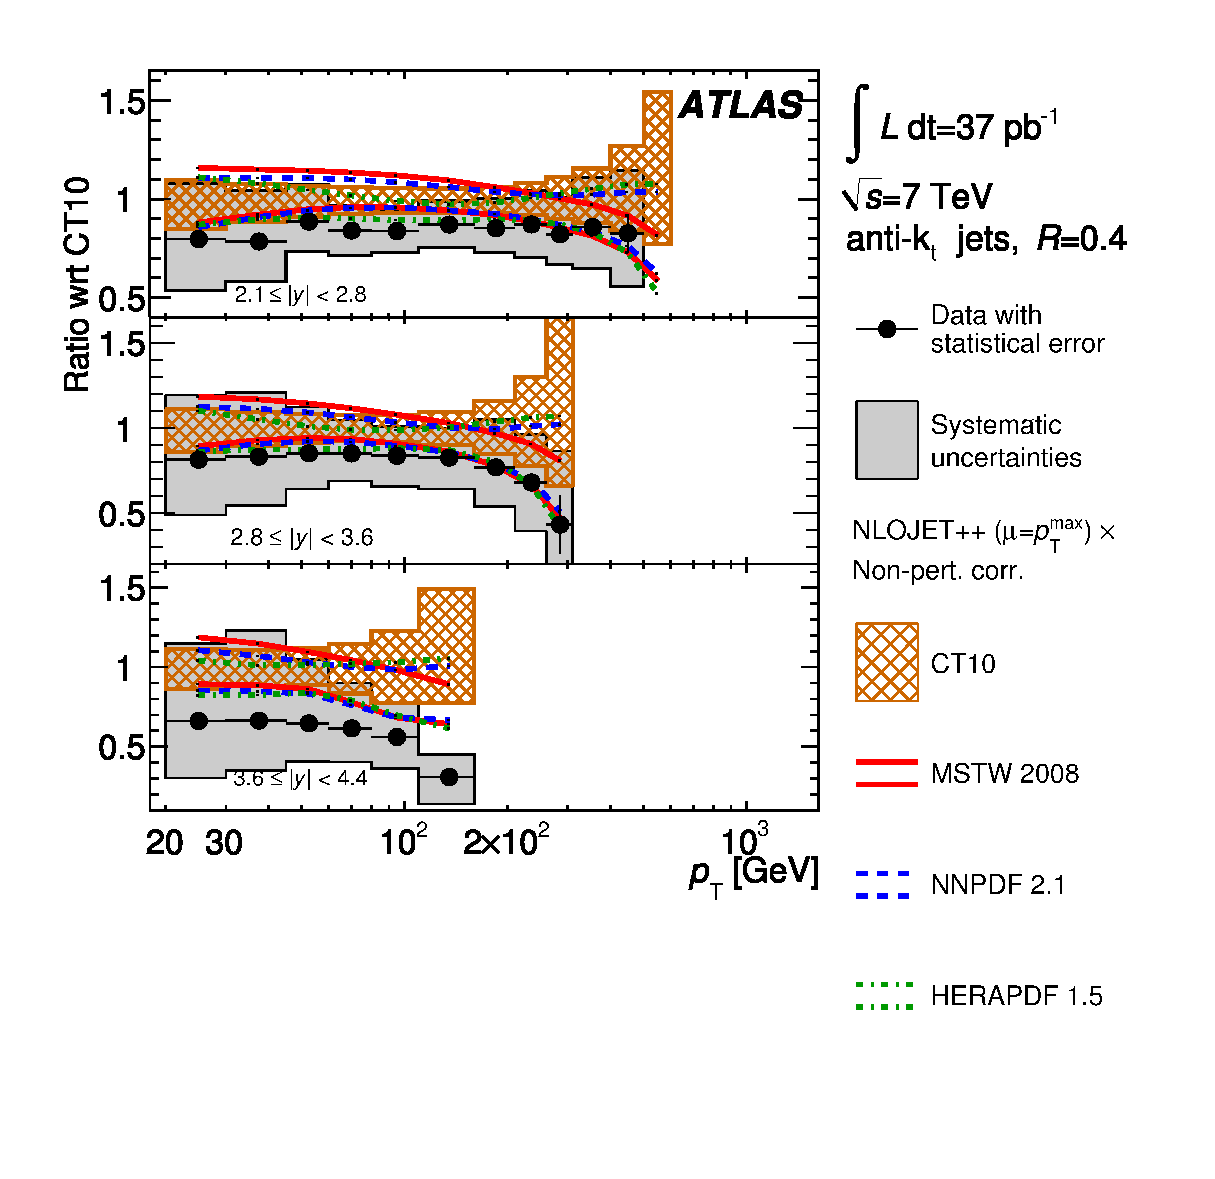
\includegraphics[width=\smallfigwidth]{chapters/forward-inclusive/InclusivePtIDSRatioForward_CT10_AntiKt04.eps}
    \label{fig:forward-inclusive:NLORatioForward_akt4}}
  \quad
  \subfloat[\Akt $R=0.6$ jets, forward rapidities]{
    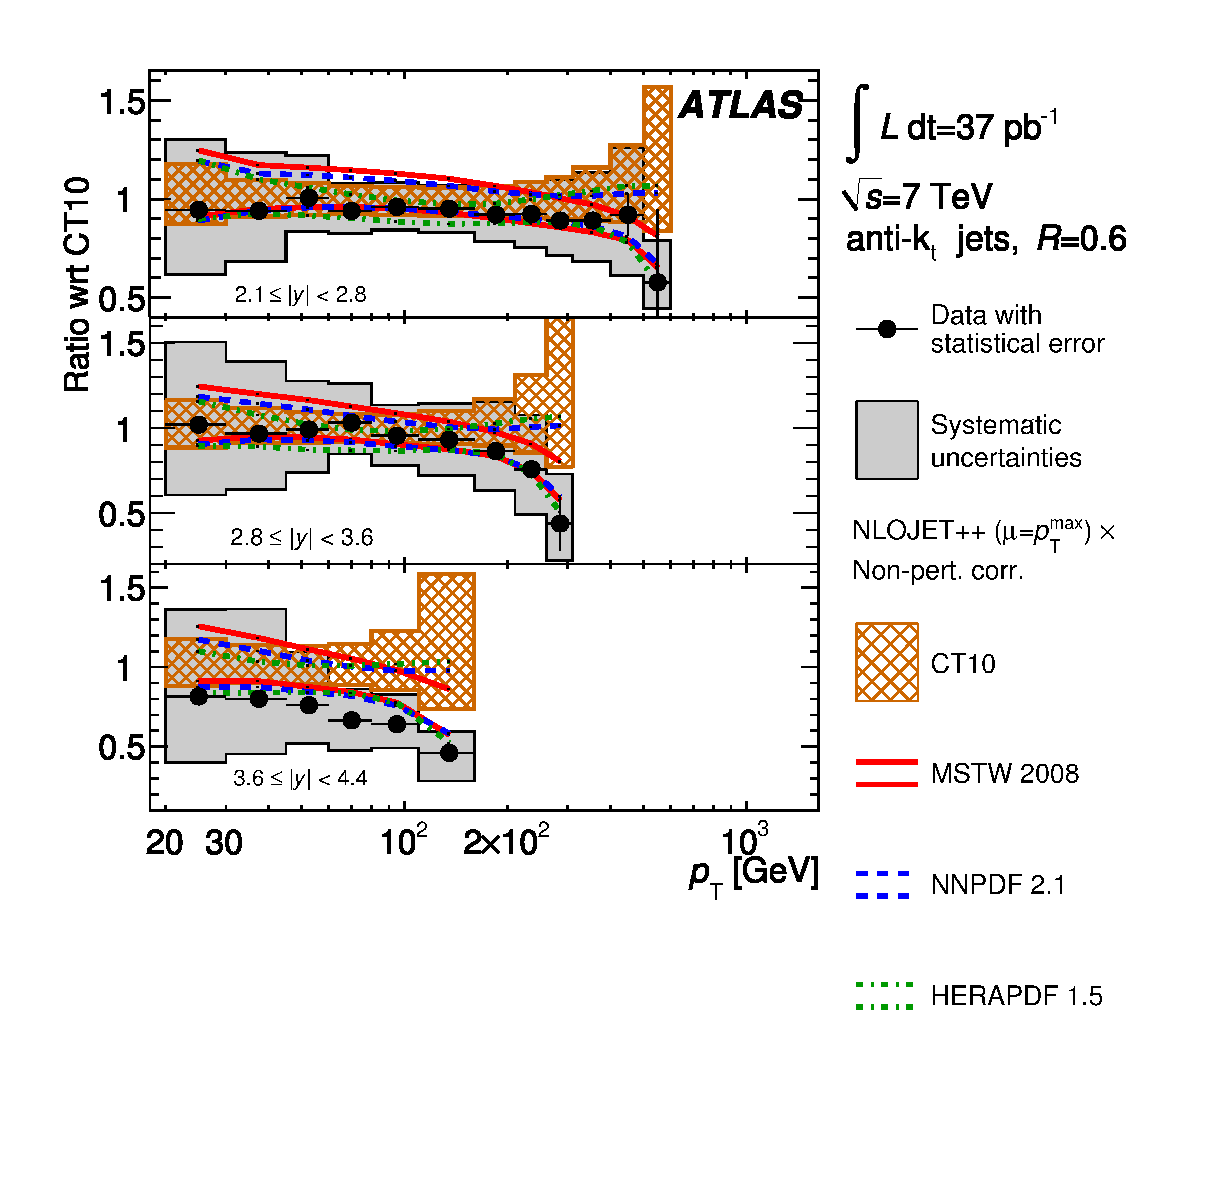
\includegraphics[width=\smallfigwidth]{chapters/forward-inclusive/InclusivePtIDSRatioForward_CT10_AntiKt06.eps}
    \label{fig:forward-inclusive:NLORatioForward_akt6}}
  \caption{Inclusive jet double-differential \xs as a function of jet
           \pT in different regions of \absRap for jets identified using the \akt
           algorithm with $R=0.4$ (left) and $R=0.6$ (right) for central rapidities (top)
           and forward rapidities (bottom). The ratio of the data
           to the theoretical prediction is shown, and the total systematic uncertainties
           on the theory and measurement are indicated. The theoretical and experimental
           uncertainties are calculated as described in \FigureRef{fig:forward-inclusive:InclusiveCrossSectionAKT4}.
           Statistically insignificant data points at large \pT are omitted in this
           ratio.}
  \label{fig:forward-inclusive:NLORatio}
\end{figure}

The comparison of the data with the \Powheg prediction, using the CT10 PDF set, is
shown for \akt jets with $R=0.4$ and $R=0.6$ in different rapidity regions in
\FigureRef{fig:forward-inclusive:PowhegRatio}. Here the data, \Powheg
predictions interfaced either \Pythia (AUET2B and \Perugia~2010 tunes) or \Herwig
(AUET2 tune) as well as fixed order \Powheg with non-perturbative corrections
are all compared. The ratio of each of these is shown with respect to the baseline NLO
\pQCD prediction, again using the CT10 PDF set.

In general, the non-perturbative corrections appear asymmetric here, particularly
at higher values of \pT since the steeply falling \xs means that, when such corrections
are applied, migrations from lower bins to higher predominate over the reverse case.
This results asymmetric shifts with respect to the nominal case, and hence an asymmetric
error band on the ratio.

\Powheg interfaced with \Pythia describes the data better than
when it is interfaced with \Herwig. Since the same matrix element is then passed through
the \Pythia and \Herwig parton showers, it can be deduced that the observable
differences between these predictions must be connected to the specifics of
their parton shower implementations and can be taken as an indication of the
uncertainty arising from the leading-logarithmic approximation used in parton
showering.

It can also be seen that the \Powheg NLO predictions, after parton shower, are in
good agreement with the pure parton level matrix element calculation from \NLOjetpp
after this has been corrected for non-perturbative effects. No direct comparison
has been carried out between the NLO parton level predictions of \Powheg and \NLOjetpp.
This is unlikely to be feasible since the \Powheg formalism guarantees to generate
the hardest third jet in the event while \NLOjetpp only guarantees that a third jet
will be generated. This is also an added complication when interfacing \Powheg with
a parton shower, as a matching process needs to be performed to ensure this condition
is adhered to.

Within the present uncertainties, the \Powheg predictions are consistent with both
the data and \NLOjetpp calculations. There is a trend for \Powheg to predict larger
\xs{s} than both the data and \NLOjetpp at low \pT, and smaller \xs{s} than \NLOjetpp (but
closer to the data) in the high-\pT region. These are also the regions where the
scale uncertainty in \NLOjetpp increases. At low \pT the non-perturbative corrections
have a significant influence, and their uncertainty can be large.

\begin{figure}[htpb]
  \subfloat[\Akt $R=0.4$ jets, central rapidities]{
    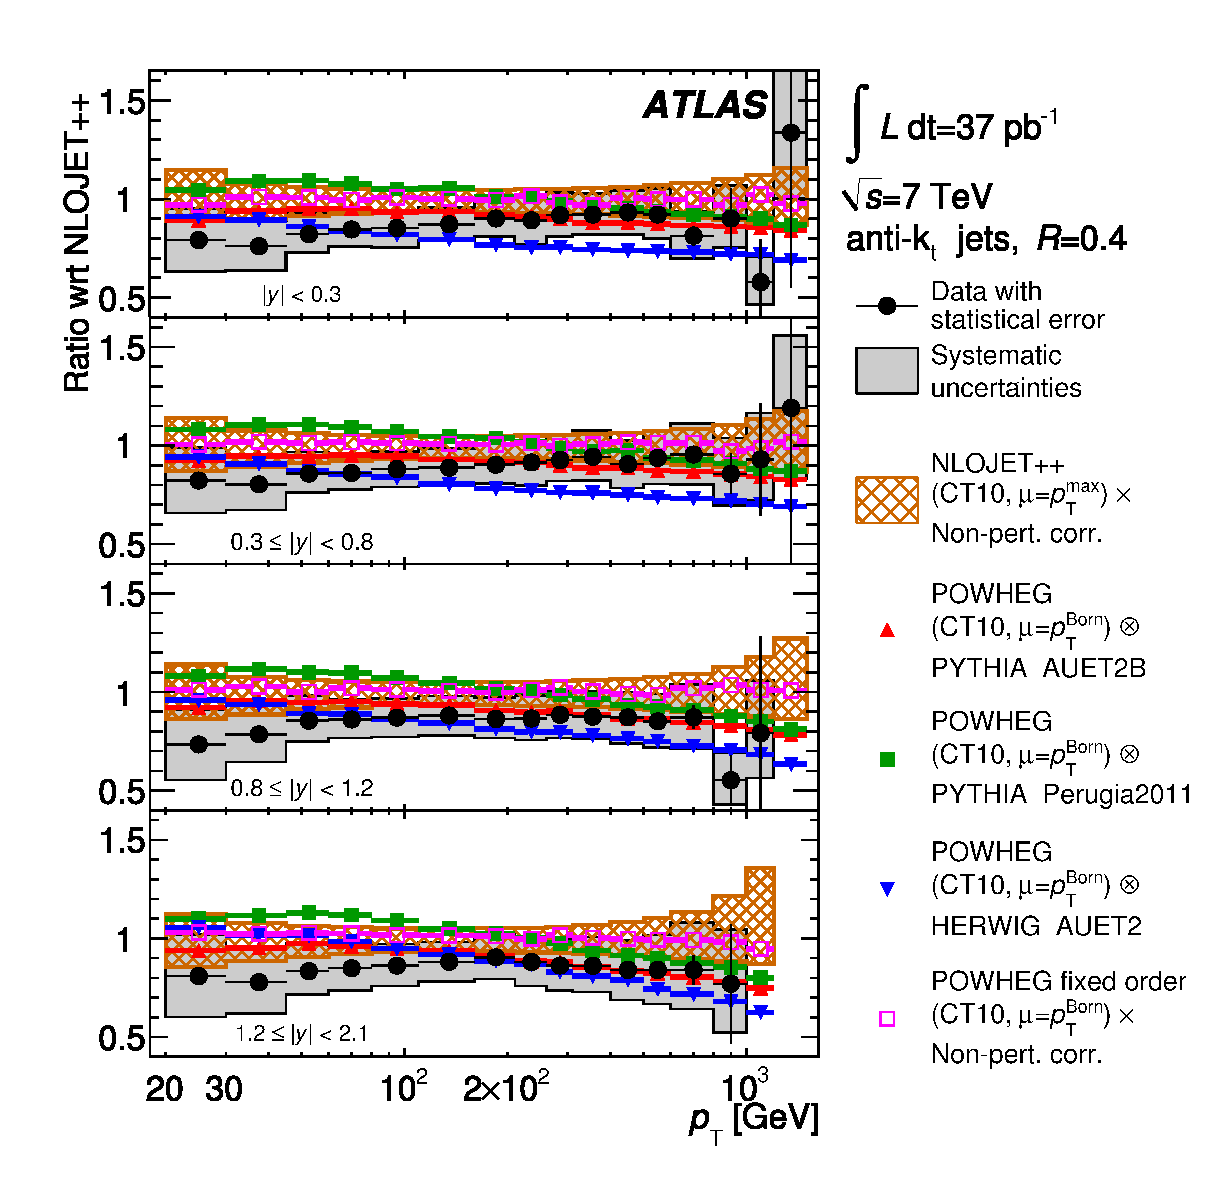
\includegraphics[width=\smallfigwidth]{chapters/forward-inclusive/InclusivePtRatioFullPowhegCentral_MSTW2008nlo90cl_AntiKt04.eps}
    \label{fig:forward-inclusive:PowhegRatioCentral_akt4}}
  \quad
  \subfloat[\Akt $R=0.6$ jets, central rapidities]{
    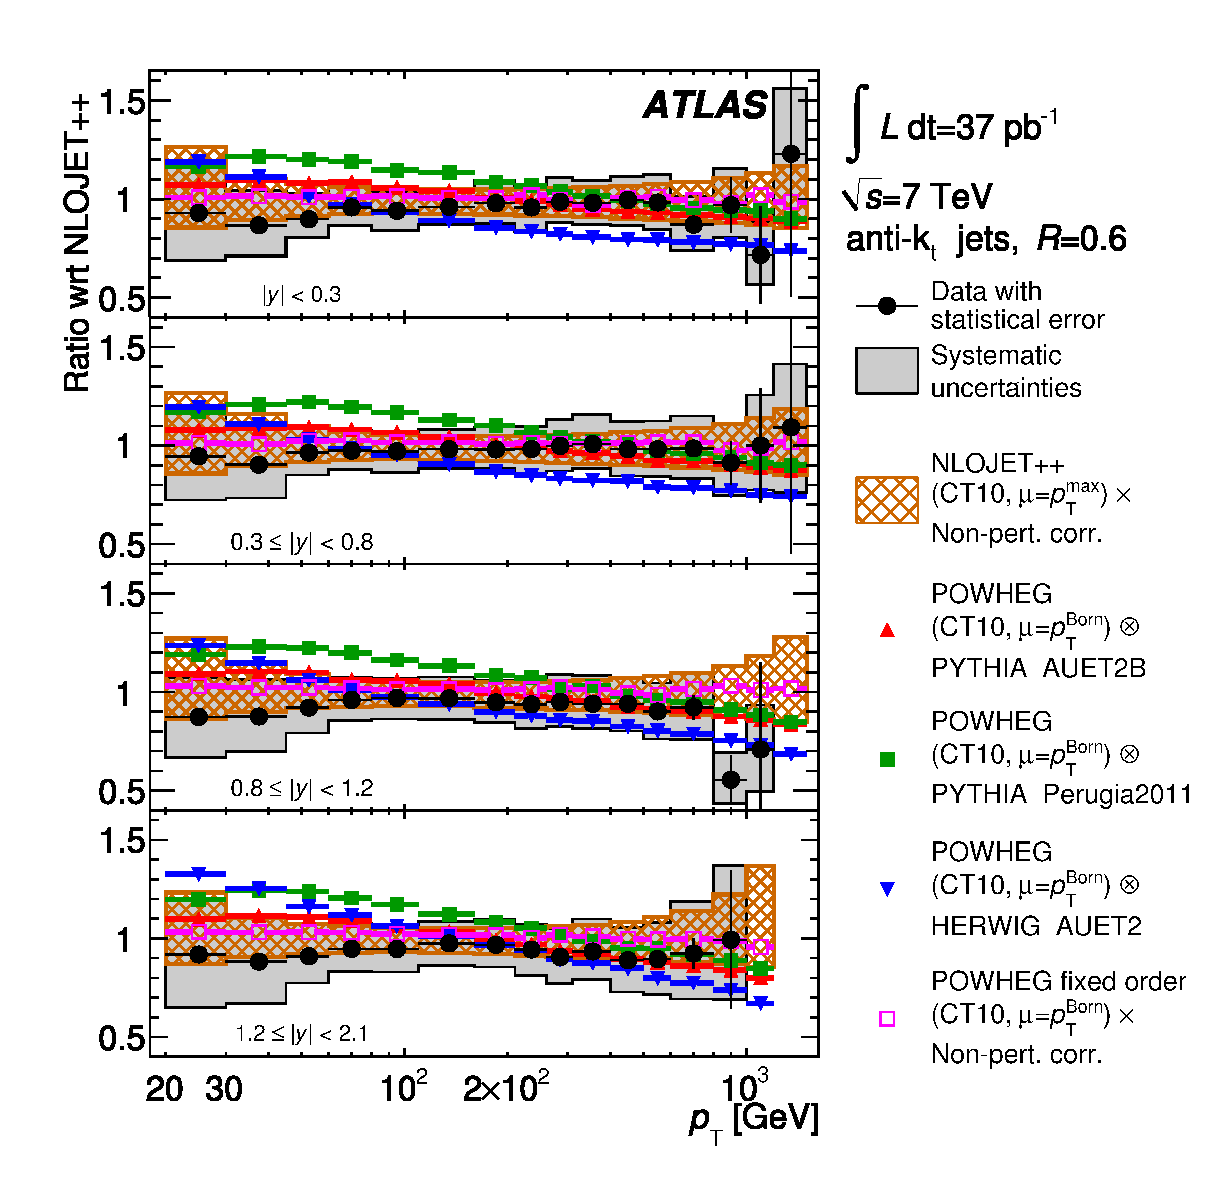
\includegraphics[width=\smallfigwidth]{chapters/forward-inclusive/InclusivePtRatioFullPowhegCentral_MSTW2008nlo90cl_AntiKt06.eps}
    \label{fig:forward-inclusive:PowhegRatioCentral_akt6}}
  \\
  \subfloat[\Akt $R=0.4$ jets, forward rapidities]{
    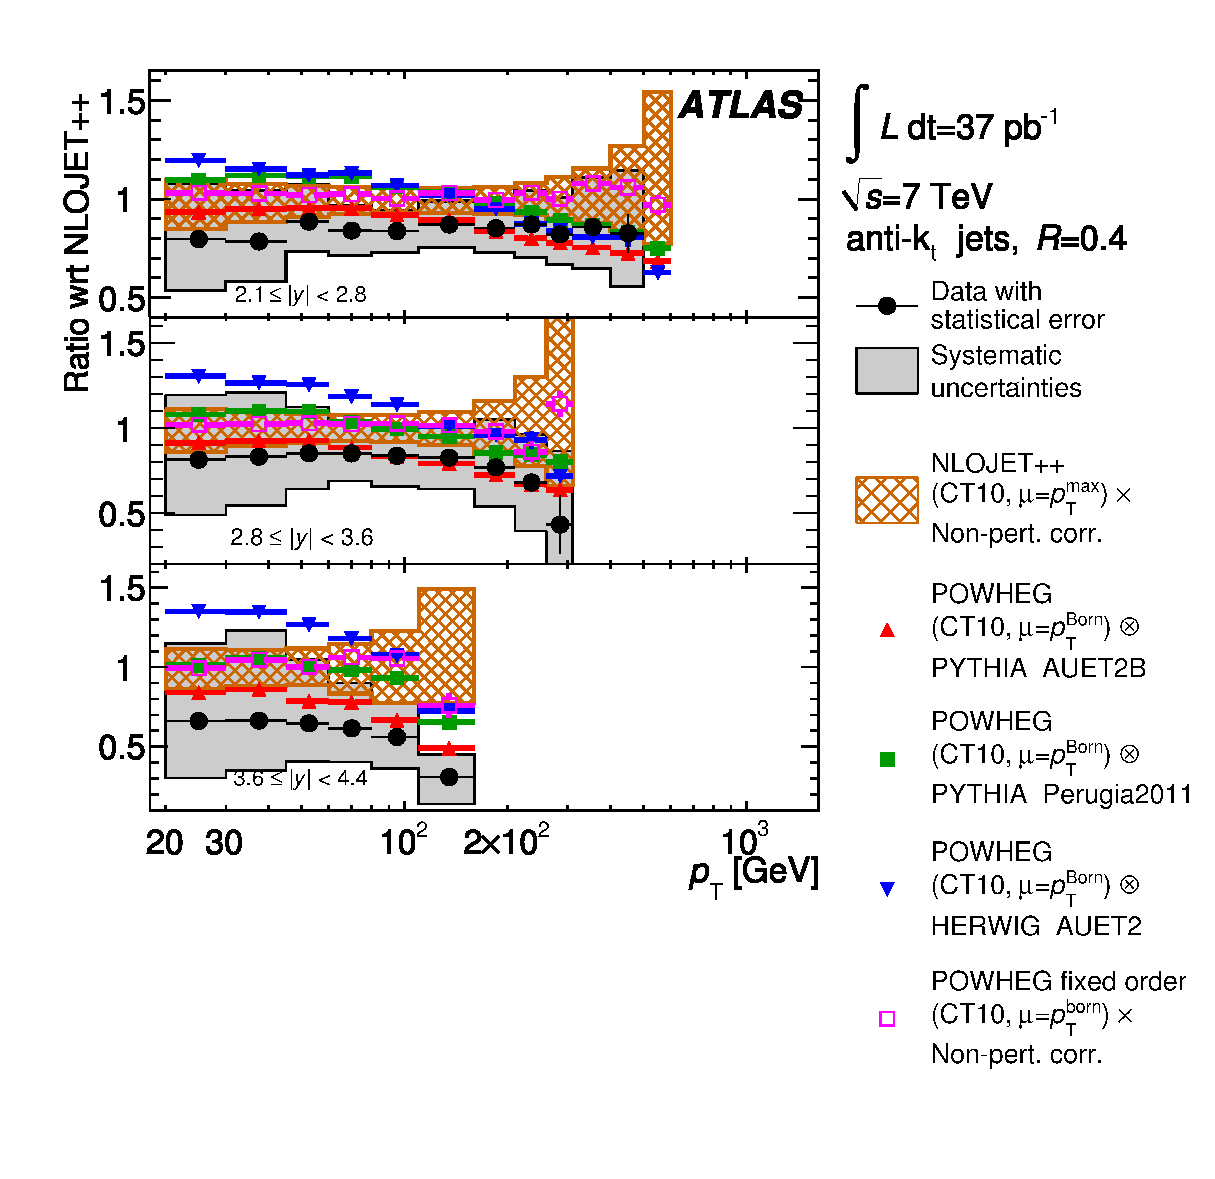
\includegraphics[width=\smallfigwidth]{chapters/forward-inclusive/InclusivePtRatioFullPowhegForward_MSTW2008nlo90cl_AntiKt04.eps}
    \label{fig:forward-inclusive:PowhegRatioForward_akt4}}
  \quad
  \subfloat[\Akt $R=0.6$ jets, forward rapidities]{
    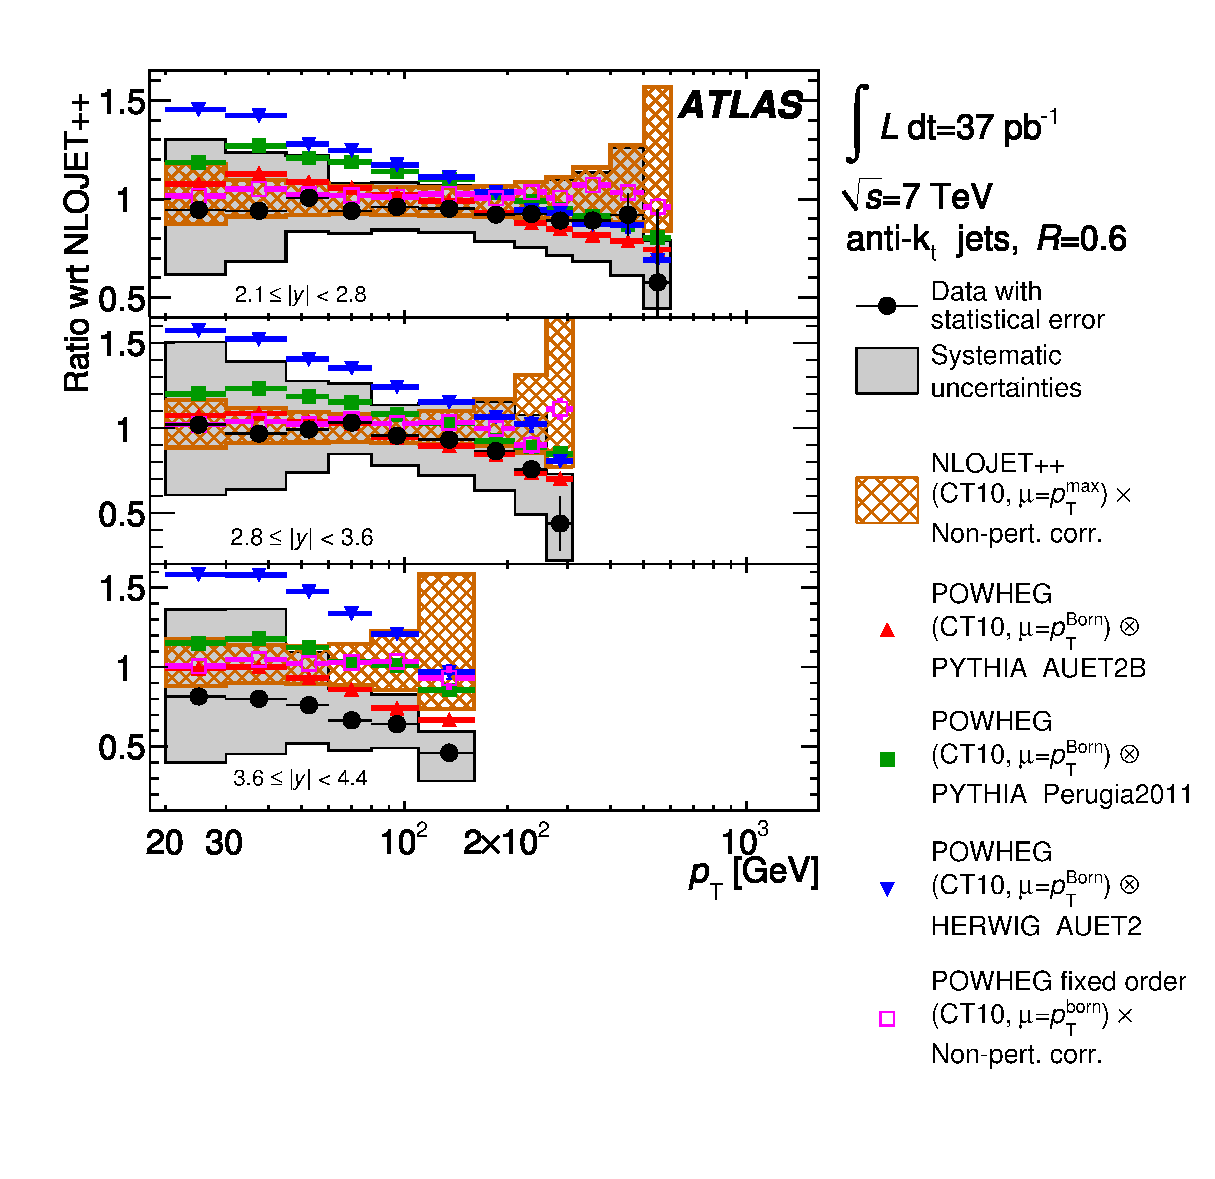
\includegraphics[width=\smallfigwidth]{chapters/forward-inclusive/InclusivePtRatioFullPowhegForward_MSTW2008nlo90cl_AntiKt06.eps}
    \label{fig:forward-inclusive:PowhegRatioForward_akt6}}
  \caption{Ratios of inclusive jet double-differential \xs to the theoretical
           prediction obtained using \NLOjetpp with the CT10 PDF set. The ratios
           are shown as a function of jet \pT in different regions of \absRap for
           jets identified using the \akt algorithm with $R=0.4$ (left) and
           $R=0.6$ (right) for central rapidities (top) and forward rapidities (bottom).
           The ratios of \Powheg predictions interfaced with
           either \Pythia or \Herwig to the \NLOjetpp predictions corrected for
           non-perturbative effects are shown and can be compared to the corresponding
           ratios for data. Only the statistical uncertainty on the \Powheg predictions
           is shown. The total systematic uncertainties on the theory and the measurement
           are indicated. The \NLOjetpp prediction and the \Powheg ME calculations
           use the CT10 PDF set. Statistically insignificant data points at large \pT
           are omitted in the ratio.}
  \label{fig:forward-inclusive:PowhegRatio}
\end{figure}


\section{Summary}
\label{sec:forward-inclusive:conclusions}
These results represent one of the most comprehensive tests of \QCD ever
performed. Data taken using minimum bias and jet triggers has been combined in
order to measure \xs{s} across a wide range of \pT and rapidity. In particular,
the forward region has never previously been explored with such precision at a
hadron collider.

Jets are reconstructed using the \akt algorithm with $R=0.4$ and $R=0.6$ in
order to probe the relative effects of the parton shower, hadronisation and
underlying event. Overall, the agreement of the NLO perturbative QCD predictions
with the measurements extends over seven orders of magnitude in \xs. These
measurements probe and may constrain the previously unexplored area of parton
distribution functions at large $x$ and high momentum transfer.

In some regions of phase space, the experimental and theoretical uncertainties
are similar in size, thereby providing some sensitivity to different
theoretical predictions. Such differences as have been observed are of the same
order as the NLO scale variation, meaning that no definitive conclusions can yet be drawn. This work has been
published in the European Physical Journal C~\cite{EPJC:2011:ATLASInclusiveJets}
and an updated version has been submitted to Physical Review D~\cite{CERN-PH-EP-2011-192}.
